\documentclass[conference]{IEEEtran}
\IEEEoverridecommandlockouts
% The preceding line is only needed to identify funding in the first footnote. If that is unneeded, please comment it out.
\usepackage{cite}
\usepackage{amsmath,amssymb,amsfonts}
\usepackage{algorithmic}
\usepackage{graphicx}
\usepackage{textcomp}
\usepackage{subfigure}


\def\BibTeX{{\rm B\kern-.05em{\sc i\kern-.025em b}\kern-.08em
    T\kern-.1667em\lower.7ex\hbox{E}\kern-.125emX}}
\begin{document}

\title{EEL 5840 Elements of Machine Intelligence\\ Project 1: Echo Cancellation\\
%{\footnotesize \textsuperscript{*}}
}

\author{\IEEEauthorblockN{Hudanyun Sheng}
\IEEEauthorblockA{\textit{Industrial and Systems Engineering} \\
\textit{University of Florida}\\
Gainesville, United States \\
hdysheng@ufl.edu}


}

\maketitle

\begin{abstract}
In this paper, the echo cancellation problem is investigated. The echo cancellation problem is viewed as an adaptive filter problem, and several different adaptive filters such as the FIR filter and the Gamma filter are introduced to accomplish the echo cancellation task. Both FIR filter and IIR filter are examined, their performance are quantified by echo return loss enhancemeng and compared. At the same time, the learning behaviour for the online learning method are studied.
\end{abstract}

\begin{IEEEkeywords}
echo cancellation, adaptive filter, FIR filter, IIR filter, Gamma filter
\end{IEEEkeywords}

\section{Introduction}

As shown in figure \ref{Diagram of the problem}, the problem is formed in this way: caller A at the near end is having some speech, which we want to here clearly, caller B at the far end, while listening, is playing music. However, due to the imperfection of two-wire to four-wire hybrid, the speech at the near end is corrupted, i.e., it is mixed with the echo from music. Our task is to remove the echo from the corrupted speech, thus to recover the speech.\\
\begin{figure}[htbp]
\centerline{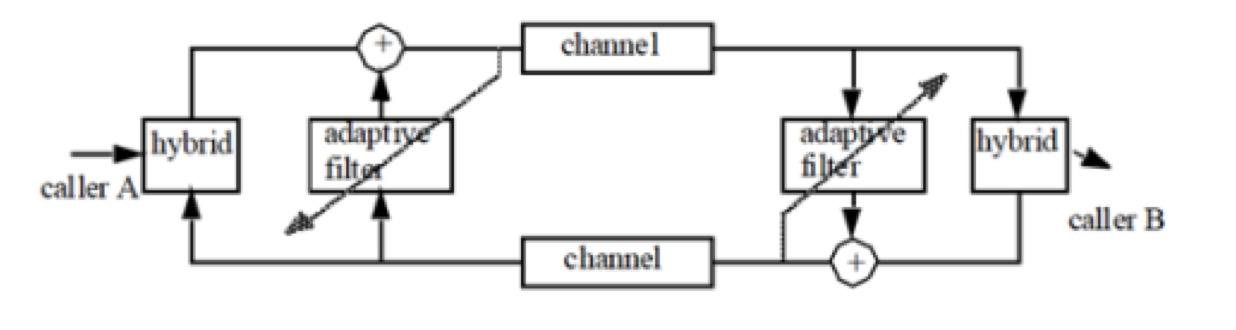
\includegraphics[width=4in]{filter.jpeg}}
\caption{Diagram of the problem.}
\label{Diagram of the problem}
\end{figure}

The echo cancellation problem can be viewed as an adaptive filter problem. The corrupted signal is given, which is the mixture of the speech and the echo; we are also given the original music signal which is the reason of the echo. And the task is to cancel the echo from the mixture, by training adaptive filter, i.e. the weight to put on the input signal. As shown in figure \ref{filter}, the $x(n)$ is the input of the filter, in our problem here it is the music signal, and $x'(n)$ represent for the echo signal, i.e. it comes from the music signal but with some complicated transforms, $v(n)$ is the speech we want to recover. The task for this filter is to mimic the way the original music signal becomes echo. In that case, the desired output $d(n)$ for our filter is the corrupted signal, which is a mixture of the echo and speech, i.e. $d(n) = x'(n) + v(n)$. After the original music signal goes through our adaptive filter, the output $y(n)$, which is ideally $x'(n)$, is compared with the desired signal $d(n)$, thus the error $e(n)$, which is the difference between desire $d(n)$ and filter output $y(n)$, is the speech $v(n)$ we want to recover. The problem was solved by minimizing the cost function.
\begin{figure}[htbp]
\centerline{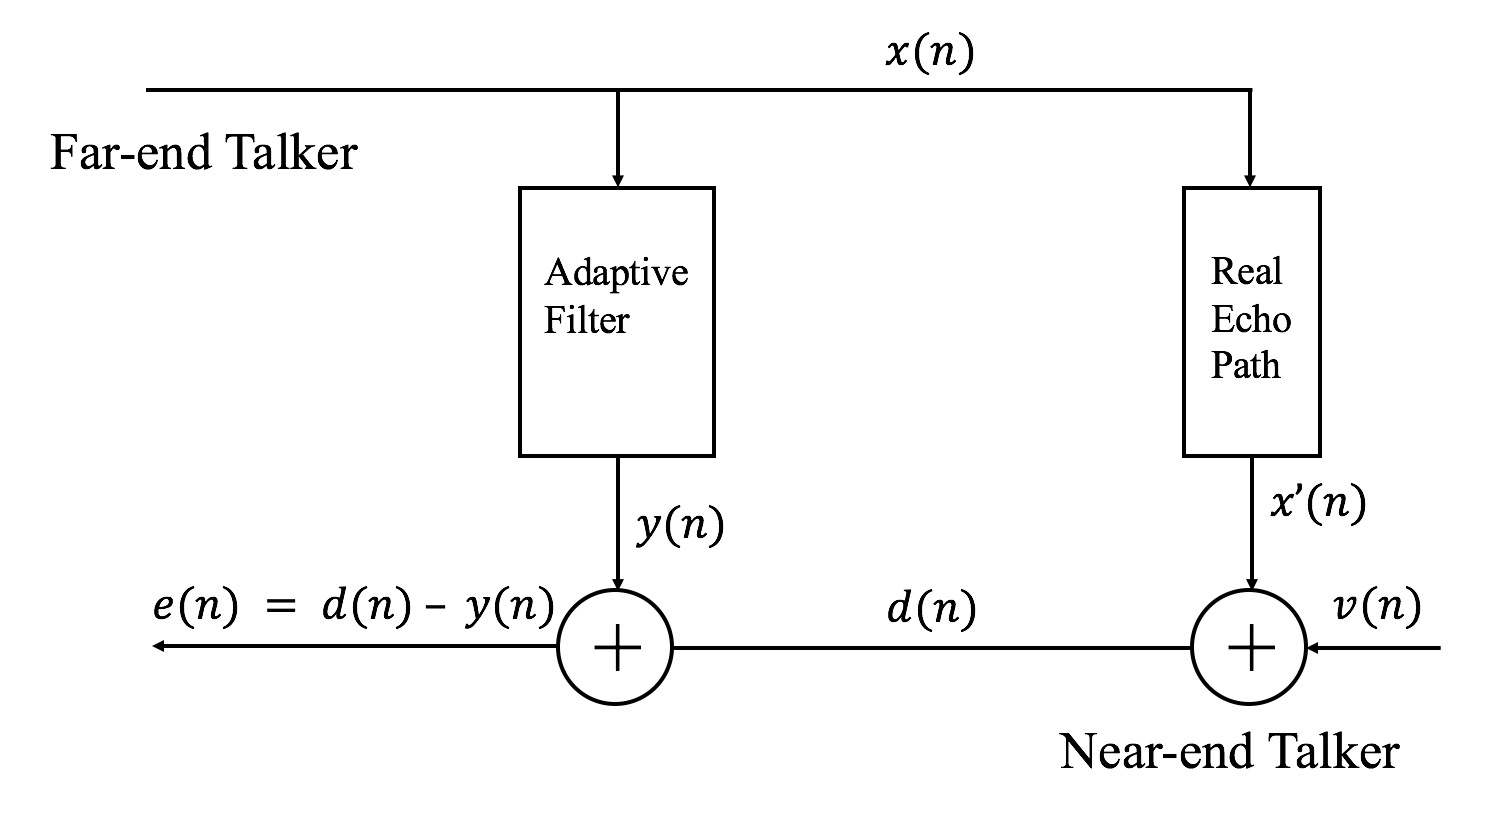
\includegraphics[width=3.5in]{FilterDiagram.jpg}}
\caption{Block diagram of the adaptive filter}
\label{filter}
\end{figure}


\section{Methodology}
	\subsection{FIR filter} FIR filters are filters with finite impulse response\cite{b1}. It is a filter whose impulse response is of finite duration. The block diagram of the FIR filter is shown in figure \ref{fir}. If we are given a set of samples $\{x_i, d_i\}$, where $x_i$ is the $i^{th}$ input sample and $d_i$ is the $i^{th}$ desired sample. The function of this mapper can be written as: $y(i) = \sum_{k=1}^{M}w_{k}x(i-k)$. The error is defined as: $e(i) = d(i) - y(i)$. And the cost function is defined: 
	\begin{equation}J(w) = \displaystyle\frac{1}{2N}\sum_{i=1}^{N}e_i^2 = \displaystyle\frac{1}{2N}\sum_{i=1}^{N}(d(i) - \sum_{k=1}^{M}w_{k}x(i-k))^2\label{eq1}\end{equation}
	And since we are having an estimization problem, given the filter order $M$, we are using the first $M$ samples to estimate the $M^{th}$ sample, i.e. the using imput samples $x(M), x(M-1),...x(1)$ to estimate the desire $x(M)$.
For the FIR filter, our task is to minimize the cost function, here we introduce two different approaches to fulfill this task.
	\begin{figure}[htbp]
	\centerline{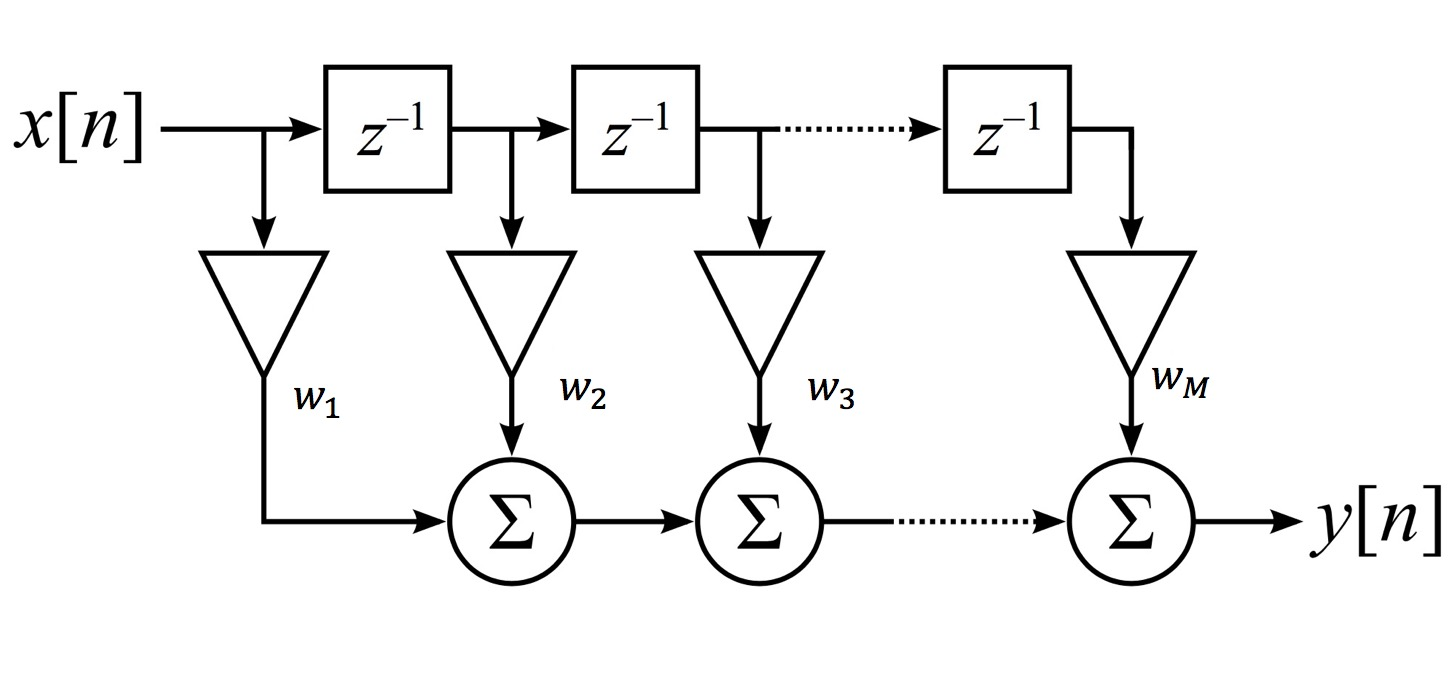
\includegraphics[width=3in]{FIRfilter.jpg}}
	\caption{Block Diagram of the FIR filter.}
	\label{fir}
	\end{figure}
		\paragraph{Wiener Solution} By taking the derivative of the cost function over the weight coefficients and set it to zero\cite{b2}, i.e. $$\frac{\partial J(w)}{\partial w} = 0$$
		we got the optimal solution for the weight coefficients: \begin{equation}w^{*} = R^{-1}P = (X^{T}X)^{-1}X^Td\label{eq2}\end{equation}
		Where $R$ is the auto-correlation matrix, and $P$ is the cross-correltation matrix. And in some case the auto-correlation matrix $R$ is not full rank, in that case, a regularization term $\lambda$ is added to the solution: 
		\begin{equation}w^{*} = (R+\lambda I)^{-1}\label{eq3}\end{equation}
		Wiener solution is an analytical solution based on the batch learning method, and is best for stationary signals. If the signal is non-stationary, the weight coefficient would be changing over time, in that case, Wiener solution would not be a suitable solution.\\
		Algorithm:\\
		 DEFINE the filter order $M$, regularization term $\lambda$\\
		COMPUTE $R$ and $P$\\
		FIND the optimal weights using $w^* = (R+\lambda I)^{-1}P$\\
		COMPUTE the error $e = d-xw^{*}$\\
	
		\paragraph{LMS Solution} Least mean squares solution learns the weight coefficients of a filter by means of gradient descent: \begin{equation}w_k(n+1) = w_k(n) + \eta \nabla J_w(n) = w_k(n) - \eta e(n)x(n)\label{eq4}\end{equation}
		Different from Wiener solution, least mean squares solution uses an online learning method, the weight coefficients are updated sample by sample in the opposite direction of the gradient. In other words, least mean squares solution learns the weight coefficients locally.Thus when it comes to non-stationary signal, the LMS solution would be a wise choice.
 For the stationary input signal, the LMS solution converges to the same optimal solution Wiener soluion get. 

To guarantee convergence, the step size should be chosen carefully - it should neither be too large to be unable to converge, nor be too small to be too slow to converge. Actually, based on \cite{b3}, the step size should not be greater than 2 over the greatest eigenvalue of the auto-correlation matrix of the input data, i.e. $\eta_{max} < \frac{2}{\lambda_{max}}$.\\

		Algorithm:\\
		 DEFINE the filter order $M$, step size $\eta$,and initial weight coefficients(zeros)\\
		FOR every sample i, compute\\
		COMPUTE: $y(i) = w^{T}x(i)$, $e(i) = d(i) - y(i)$, $J(i) = e^{2}(i)$\\
		UPDATE: $\hat w = w+2\mu e(i)x(i)$

	\subsection{IIR filter} IIR filters are filters with infinite impulse response\cite{b4}. Different from FIR filters, the IIR filters have the feedback, which means a larger filter memory compared to the FIR filter with the same filter order.
		\paragraph{The Gamma Filter} As one example of the IIR filter, the Gamma filter is defined as\cite{b5}:
		\begin{equation}y(n) = \sum_{k=0}^{M}w_kx_k(n)\label{5}\end{equation}
	where $x_k(n)=(1-\mu)x_k(n-1) + \mu x_{k-1}(n-1)$, $k = 1,...,M$. $x_0(n) = x(n)$ is the input signal and $y(n)$ is the output signal, where $\mu$ is the feedback parameter. The block diagram the the Gamma filter is shown in figure \ref{diagramGamma}. When $\mu = 1$, the Gamma filter is the same as the FIR filter with the same filter order. 
			Algorithm:\\
		 DEFINE the filter order $M$, step size $\eta$, feedback parameter $\mu$, and initial weight coefficients(zeros)\\
		FOR every sample i, compute\\
		FOR every $k = 1,..., M$:\\
		COMPUTE $x_k(i) = (1-\mu)x_{k}(i-1) + \mu x_{k-1}(i-1)$,
		END\\
		COMPUTE $y(i) = w^{T}x_k(i)$, $e(i) = d(i) - y(i)$, $J(i) = e^{2}(i)$\\
		END\\
		UPDATE $\hat w = w+2\mu e(i)x(i)$
	\begin{figure}[tbp]
	\centerline{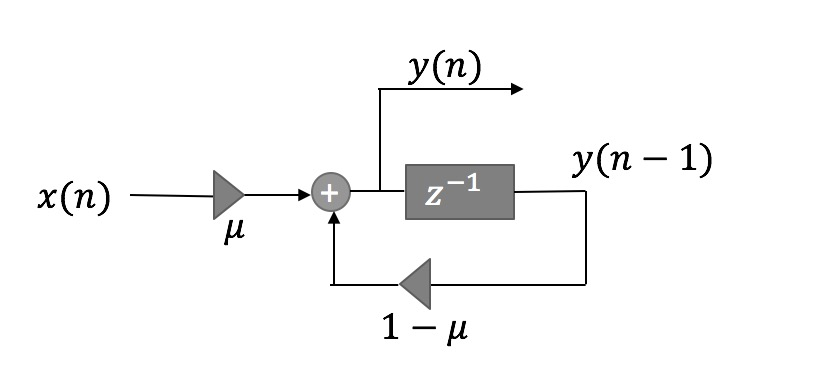
\includegraphics[width=3in]{gammafilterblock.jpg}}
	\caption{The block diagram of the Gamma filter}
	\label{diagramGamma}
	\end{figure}
	
	\subsection{Echo Return Loss Enhancement} Echo return loss enhancement (ERLE) is the amount of additional signal loss applied by the echo canceller, it can be used as an quantitative measure of how well the echo is being canceled. It is defined as:
	\begin{equation}ERLE = 10log_{10}\displaystyle\frac{\frac{1}{N}\sum_{i=1}^{N}d_i^2}{\frac{1}{N}\sum_{i=1}^{N}e_i^2} = 10log_{10}\displaystyle\frac{\sum_{i=1}^{N}d_i^2}{\sum_{i=1}^{N}e_i^2}\label{6}\end{equation}
And basically, minimize the cost function is equilvalent to maximize the ERLE, so we want the value of ERLE to be large. But in our case, the error term is the speech we want to recover, what we are minimizing is the difference between the learned echo and the real echo. So the error term would not converge to 0, but to a fixed value.
	
	
\section{Results}
	\subsection{FIR filter}
		\paragraph{Wiener Solution} To examine whether the signal we are dealing with is stationay or not, the Wiener solution is performed. The number of taps is changed from 5 to 100 in steps of 5, and with every fixed number of taps, the regularization term is changed from 0 to 0.5 in steps of 0.01. Based on the experiment, the minimum MSE is obtained at filter order $100$ and regularization term $\lambda= 0$. And the Wiener filter can get the maximum ERLE value of 8.3208. Figure \ref{fig1} left shows the comparison regarding two parameters. Figure \ref{fig1} right shows the ERLE curve of the Wiener filter as adaptation as a function of the number of taps. 
		
What is more, if open different windows, the Wiener filter would got different result of weight coefficients because of the non-stationarity of the signal we are dealing with. One example is shown here: with the same window width 50000, the first window has a starting point at 5, while the second window has a starting point at 140000, and figure \ref{fig2} shows the zoomed result of the weight coefficient gained by Wiener filter for both of the two windows.


	\begin{figure}[htbp]
	\centering
	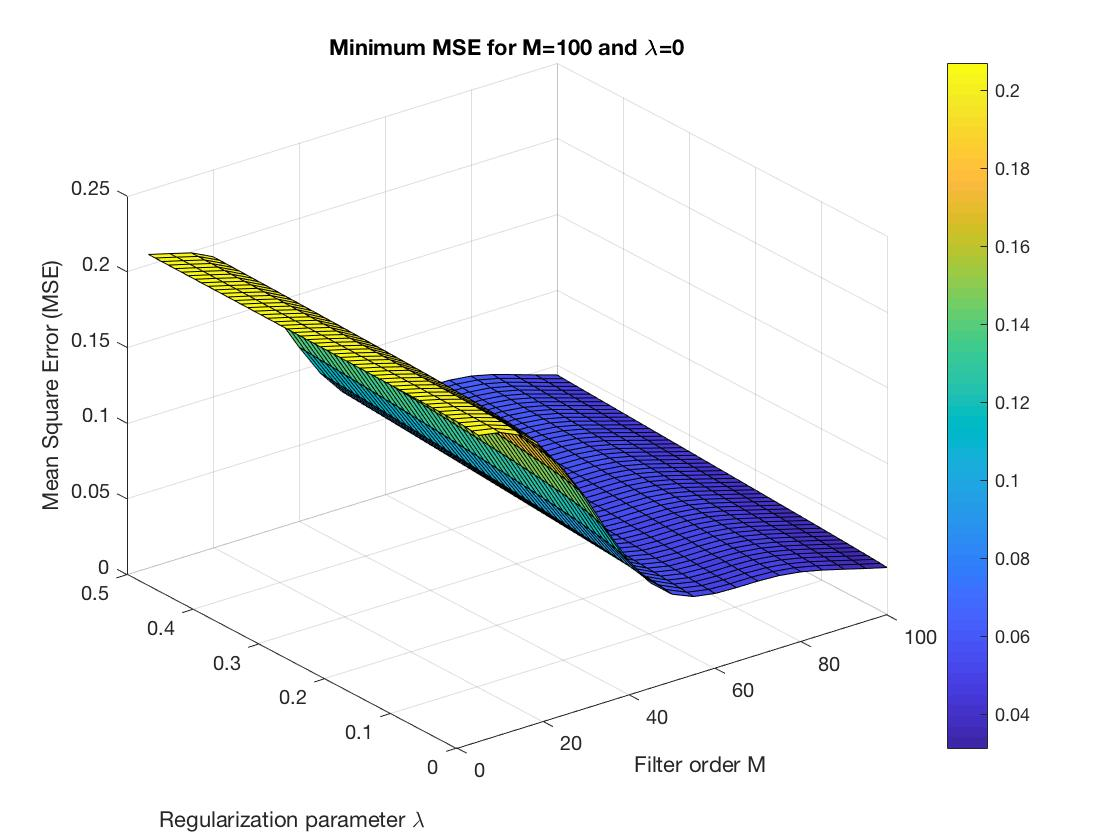
\includegraphics[width = 1.7in]{Wiener2paracom.jpg}
	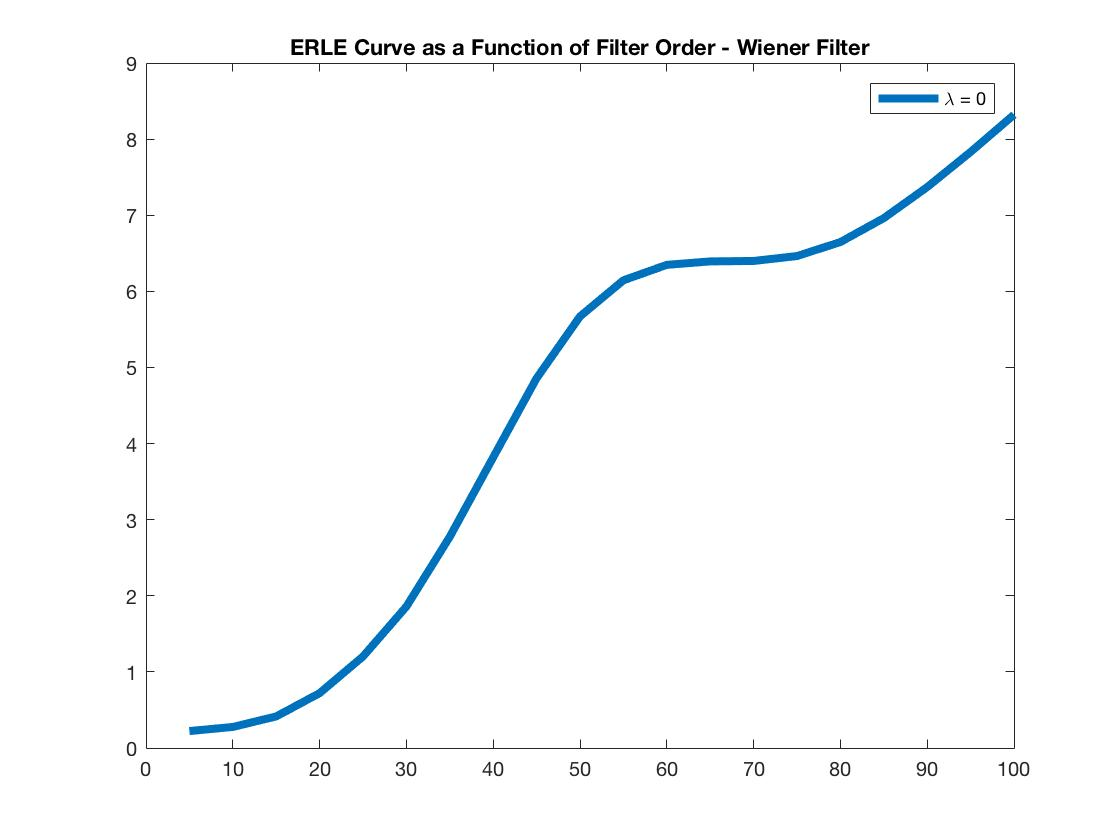
\includegraphics[width=1.7in]{WienerERLE.jpg}
	\caption{Left: The 3D surface of the MSE when changing both filter order and regularization term together. Right: The ERLE curve of the Wiener filter as adaptation as a function of the 	number of taps. The maximum ERLE value is 8.3208 and is gained at $\lambda = 0$ and $M = 100$.}
	\label{fig1}
	\end{figure}


	\begin{figure}[htbp]
	\centering
	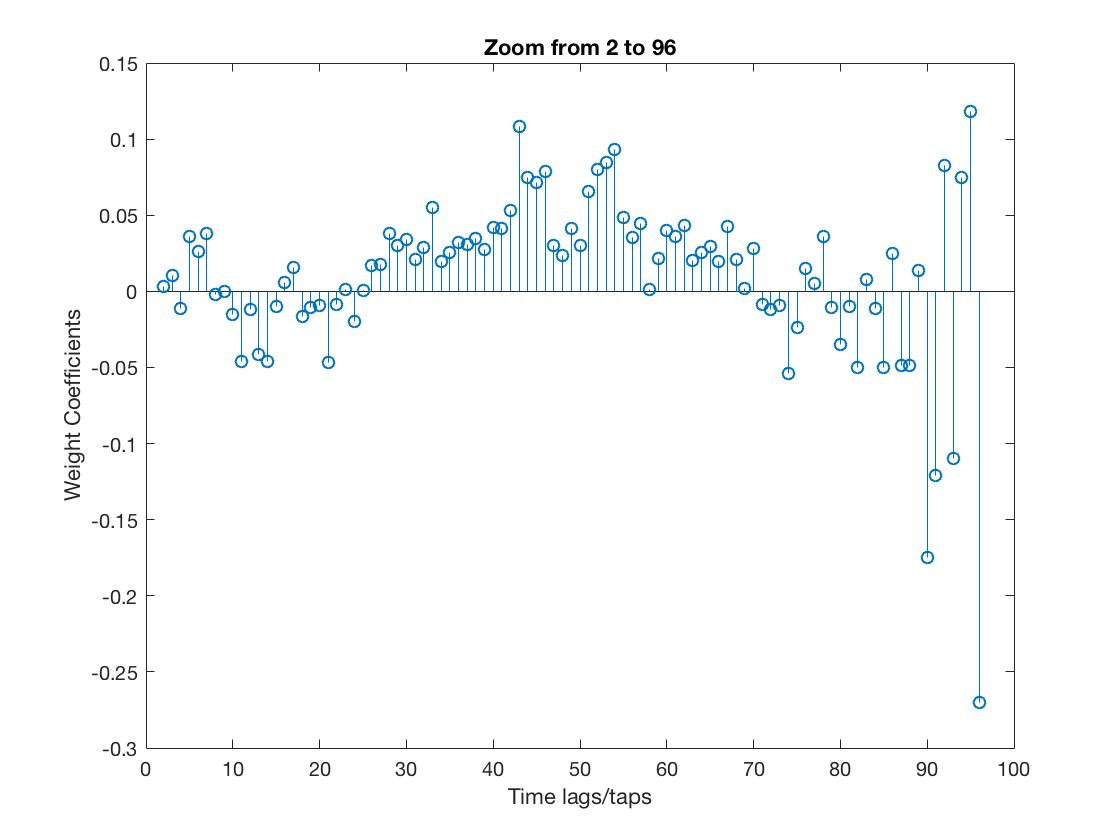
\includegraphics[width = 1.7in]{Wiener_w1_weight_zoom.jpg}
	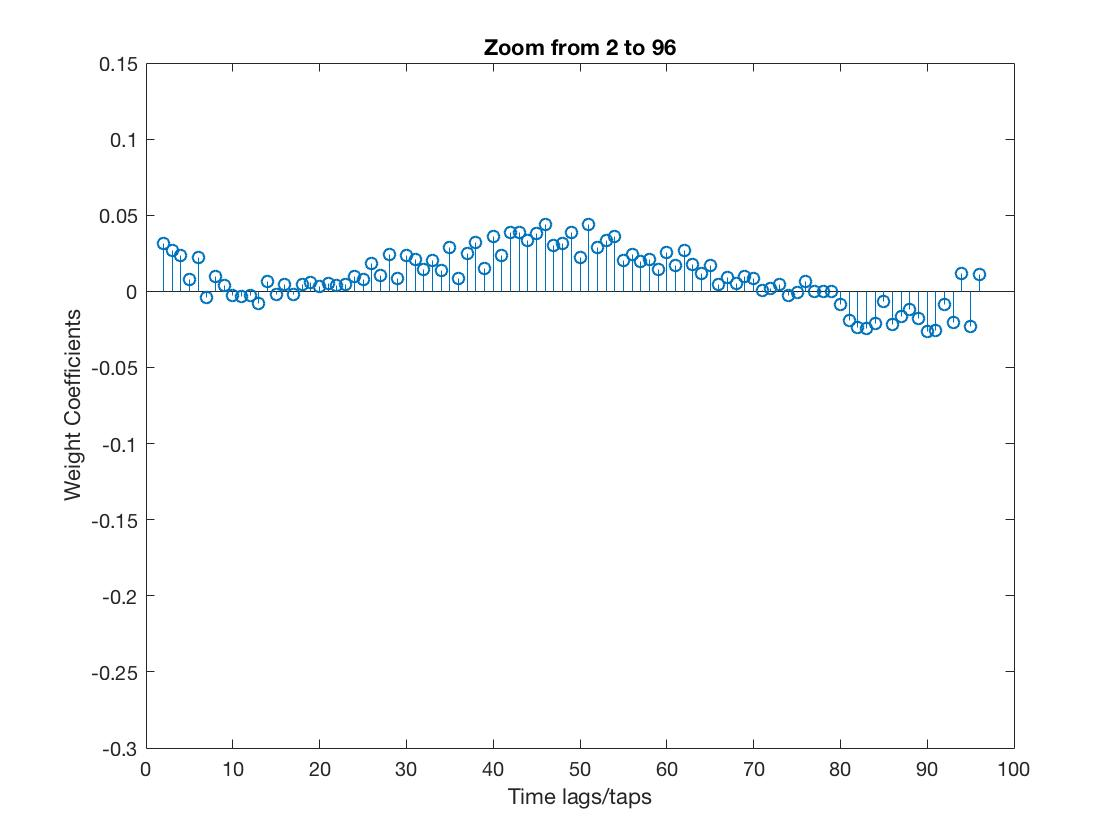
\includegraphics[width=1.7in]{Wiener_w2_weight_zoom.jpg}
	\caption{Left: The weight coefficient of 1st window with Wiener Filter. Right: The weight coefficient of 2nd window with Wiener Filter.}
	\label{fig2}
	\end{figure}


		\paragraph{LMS Solution} The step sizes $\eta$ were chosen from $\{{10^{-6}, 5\times 10^{-5}, 10^{-5}, 5\times 10^{-4},10^{-4}, 10^{-3}}\}$, and with every fixed the step size, the number of taps are changed from 5 to 100 in steps of 5, the ERLE curve after several iterations is shown in figure \ref{ERLELMS}. With different step size, we got the same result of what the best filter order is - the best filter order of LMS solution with a linear FIR filter is 100. 
	
	\begin{figure}[htbp]
	\centerline{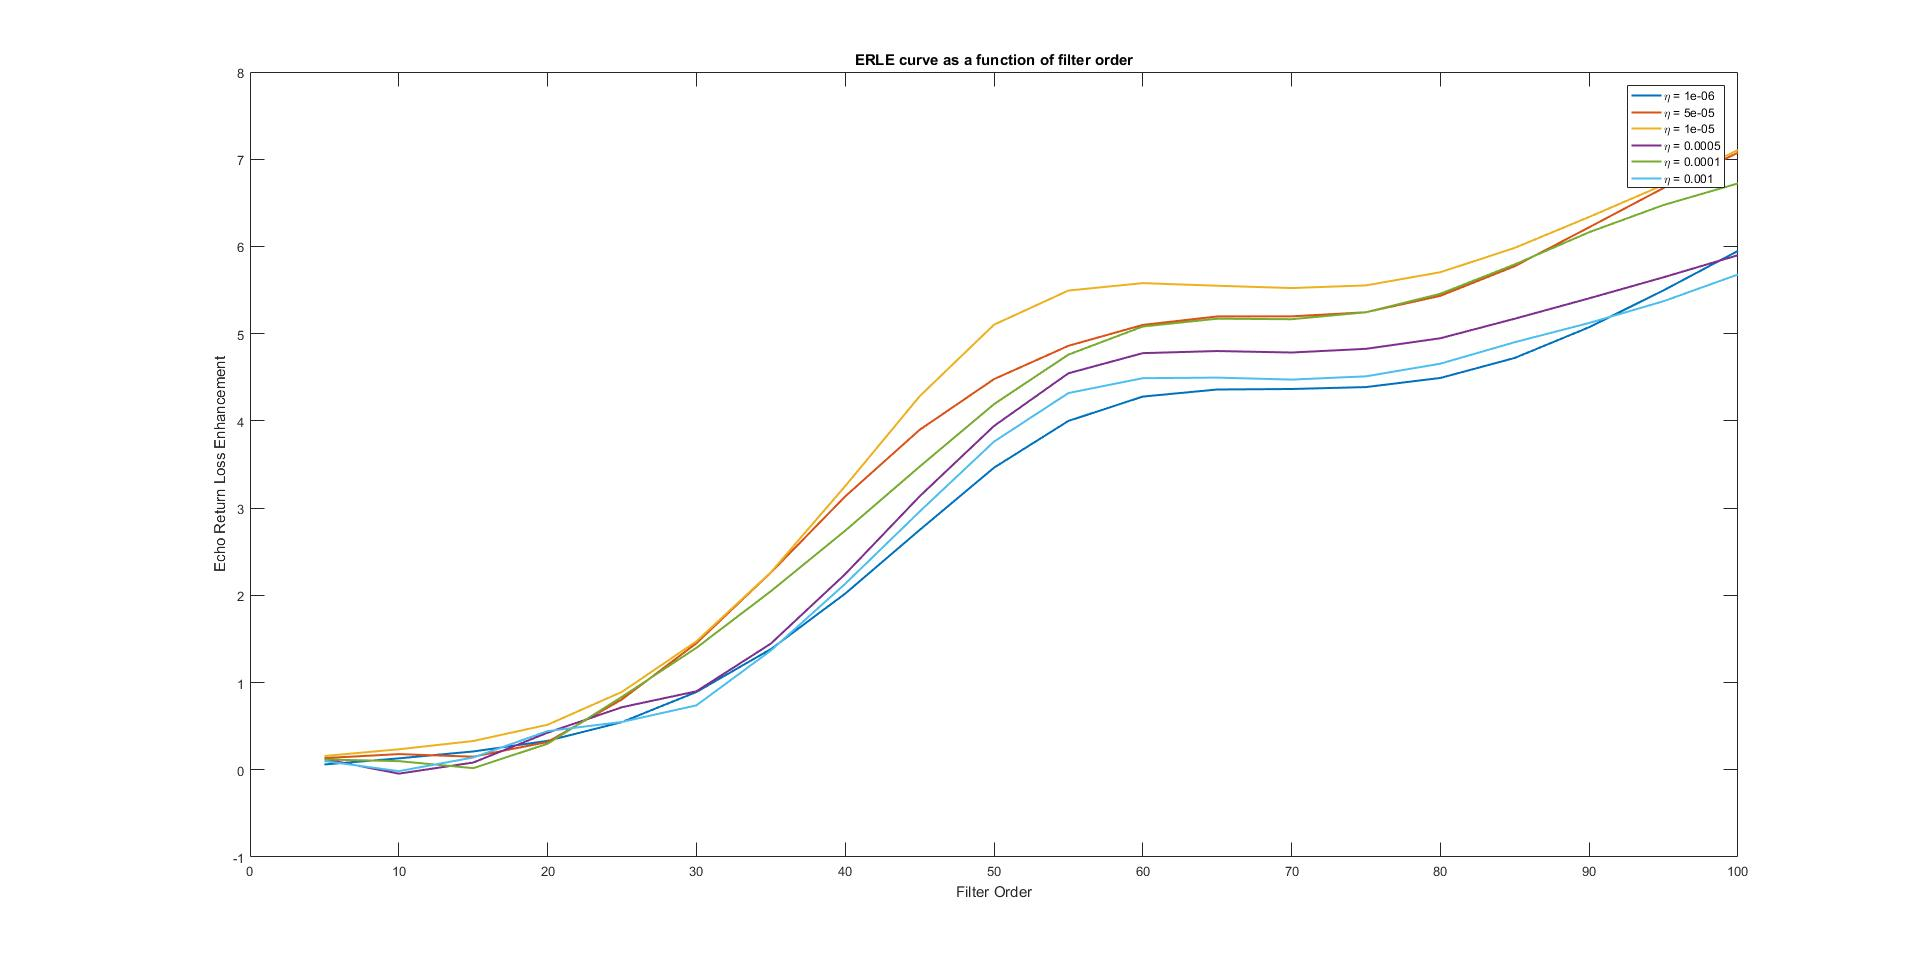
\includegraphics[width=3.5in]{LMS_ERLE.jpg}}
	\caption{The ERLE curve of the FIR filter after adaptation as a function of the number of taps. With different step sizes, the values of ERLE gets the maximum when the filter order is 100. And with step size $10^{-5}$, it gets the maximum ERLE 7.1052.}
	\label{ERLELMS}
	\end{figure}

	With the best filter order found, what to do next is to fix this filter order and changing the step size $\eta$ to select the best one. The learning curves with different step size are shown in figure \ref{LMSlcALL}. And the selected learning curves as well as their weight tracks are shown in figures \ref{LMSeta1} to  \ref{LMSeta6}.
	\begin{figure}[htbp]
	\centerline{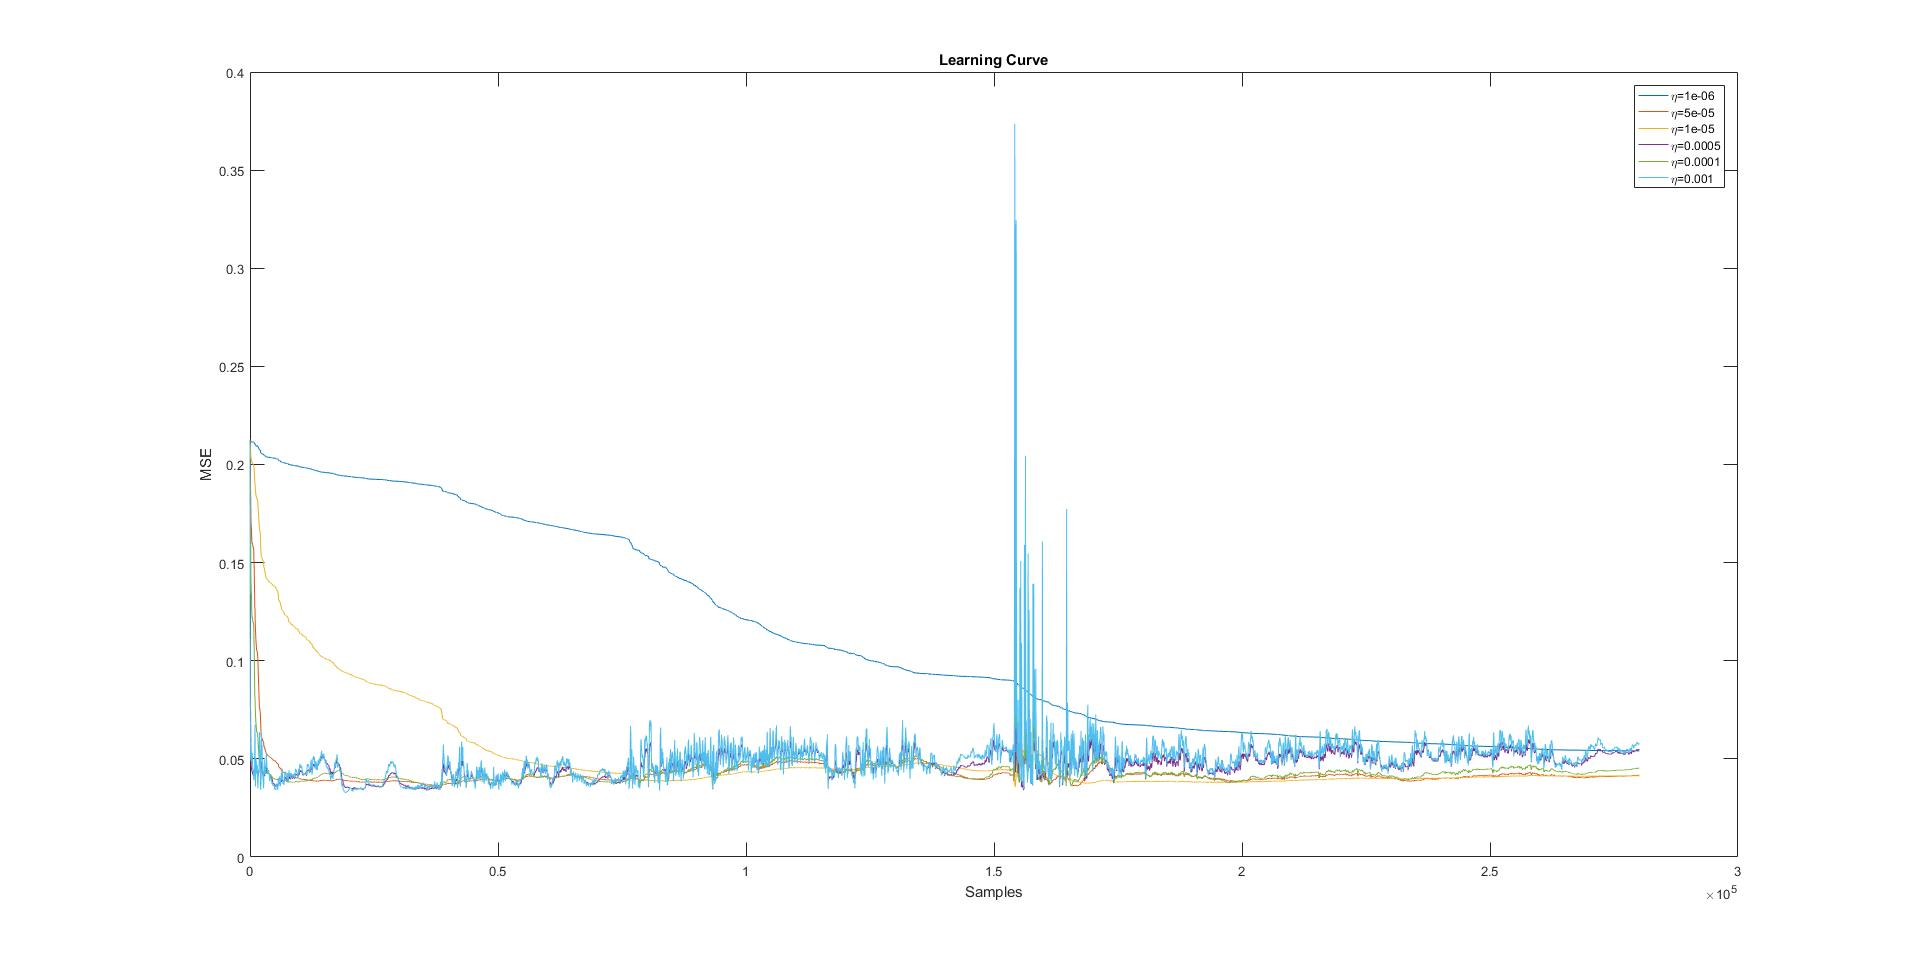
\includegraphics[width=3.5in]{LMS_LC_All.jpg}}
	\caption{The comparison of learning curves with different step sizes - LMS filter.}
	\label{LMSlcALL}
	\end{figure}
	
	\begin{figure}[htbp]
	\centering
	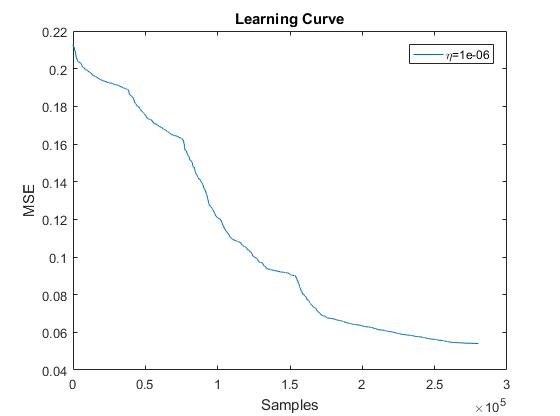
\includegraphics[width = 1.7in]{LMS_LC_eta6.jpg}
	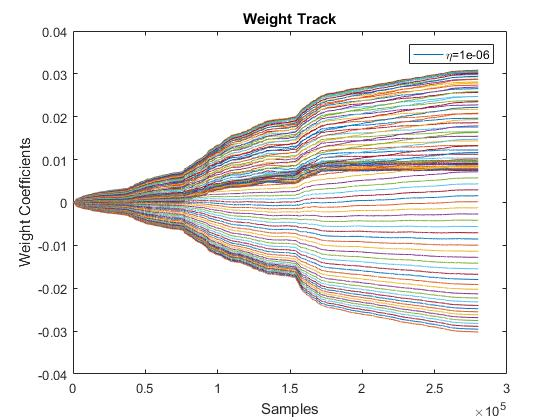
\includegraphics[width=1.7in]{LMS_WT_1.jpg}
	\caption{Left: The learning curve of LMS filter with step size $\eta = 10^{-6}$ . Right: The weight track of LMS filter with step size $\eta = 10^{-6}$.}
	\label{LMSeta1}
	\end{figure}

	\begin{figure}[htbp]
	\centering
	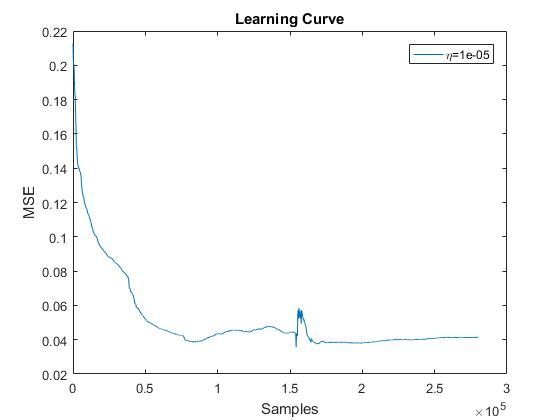
\includegraphics[width = 1.7in]{LMS_LC_eta4.jpg}
	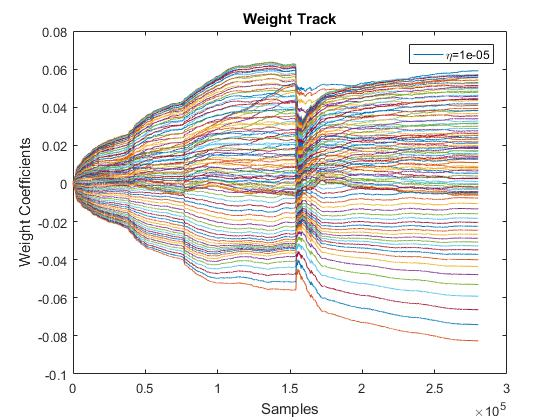
\includegraphics[width=1.7in]{LMS_WT_3.jpg}
	\caption{Left: The learning curve of LMS filter with step size $\eta = 5\times 10^{-5}$ . Right: The weight track of LMS filter with step size $\eta =10^{-5}$.}
	\label{LMSeta2}
	\end{figure}

	\begin{figure}[htbp]
	\centering
	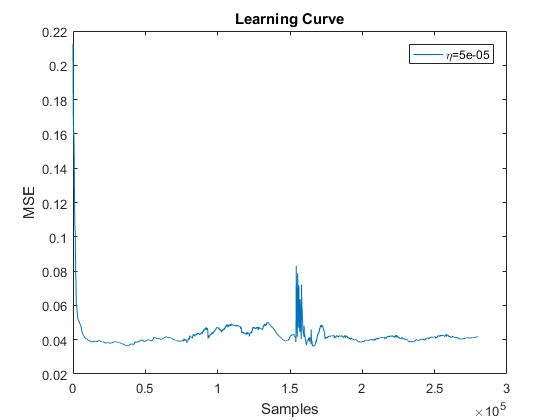
\includegraphics[width = 1.7in]{LMS_LC_eta5.jpg}
	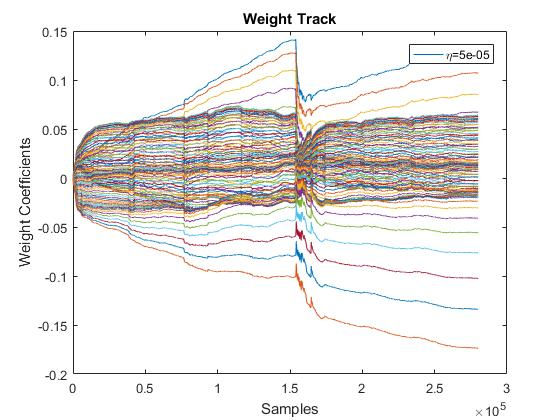
\includegraphics[width=1.7in]{LMS_WT_2.jpg}
	\caption{Left: The learning curve of LMS filter with step size $\eta = 10^{-5}$ . Right: The weight track of LMS filter with step size $\eta =  5\times 10^{-5}$.}
	\label{LMSeta3}
	\end{figure}

	\begin{figure}[htbp]
	\centering
	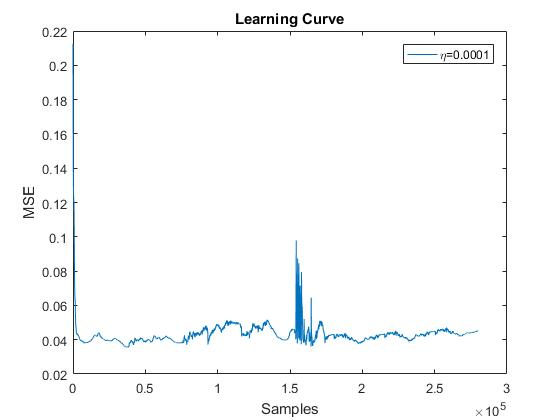
\includegraphics[width = 1.7in]{LMS_LC_eta2.jpg}
	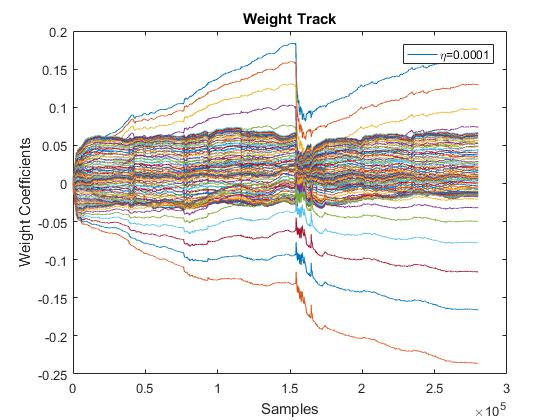
\includegraphics[width=1.7in]{LMS_WT_5.jpg}
	\caption{Left: The learning curve of LMS filter with step size $\eta = 5\times 10^{-5}$ . Right: The weight track of LMS filter with step size $10^{-4}$.}
	\label{LMSeta4}
	\end{figure}

	\begin{figure}[htbp]
	\centering
	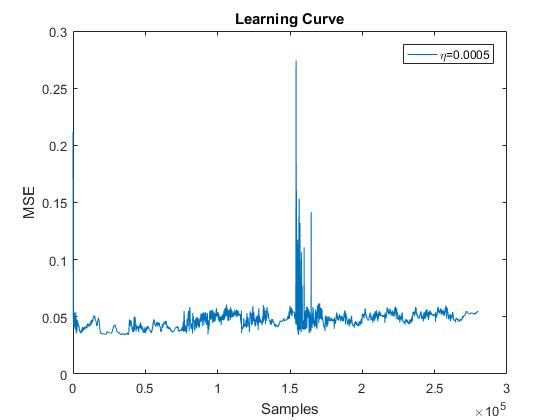
\includegraphics[width = 1.7in]{LMS_LC_eta3.jpg}
	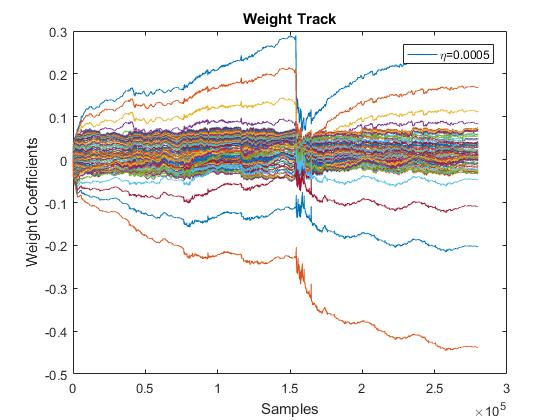
\includegraphics[width=1.7in]{LMS_WT_4.jpg}
	\caption{Left: The learning curve of LMS filter with step size $\eta = 10^{-4}$ . Right: The weight track of LMS filter with step size $\eta =  5\times 10^{-4}$.}
	\label{LMSeta5}
	\end{figure}

	\begin{figure}[htbp]
	\centering
	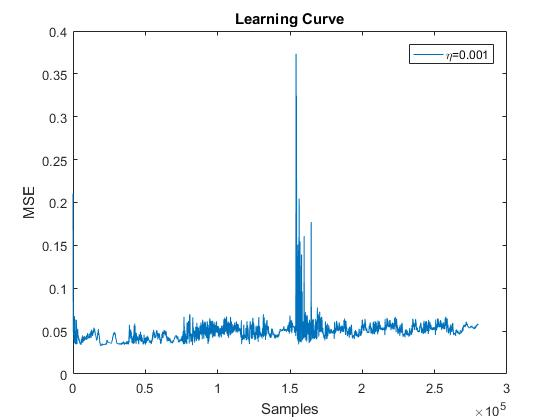
\includegraphics[width = 1.7in]{LMS_LC_eta1.jpg}
	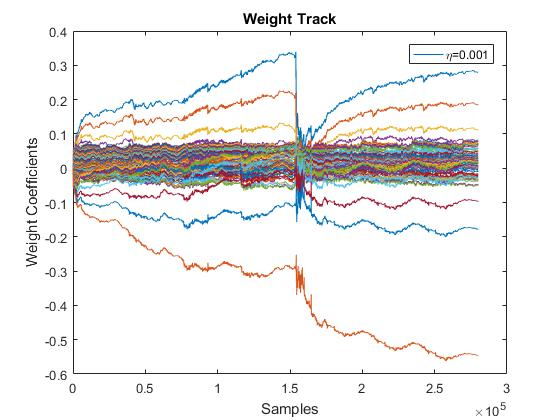
\includegraphics[width=1.7in]{LMS_WT_6.jpg}
	\caption{Left: The learning curve of LMS filter with step size $\eta = 10^{-4}$ . Right: The weight track of LMS filter with step size $\eta = 0.001$.}
	\label{LMSeta6}
	\end{figure}


	\subsection{IIR filter}
		\paragraph{Gamma Filter}  Wishing to find the best filter order with the feedback parameter in the tap delay line $\mu$ fixed to be 0.2, different step sizes are fixed with the number of taps changing from 5 to 100 in steps of 5 for each one fixed step size. The step sizes are chosen from $\{ 0.01, 0.005, 0.001, 0.0005, 0.0001\}$, the corresponding ERLE curves are shown in figure \ref{ERLEGammaall}.
		
	\begin{figure}[tbp]
	\centerline{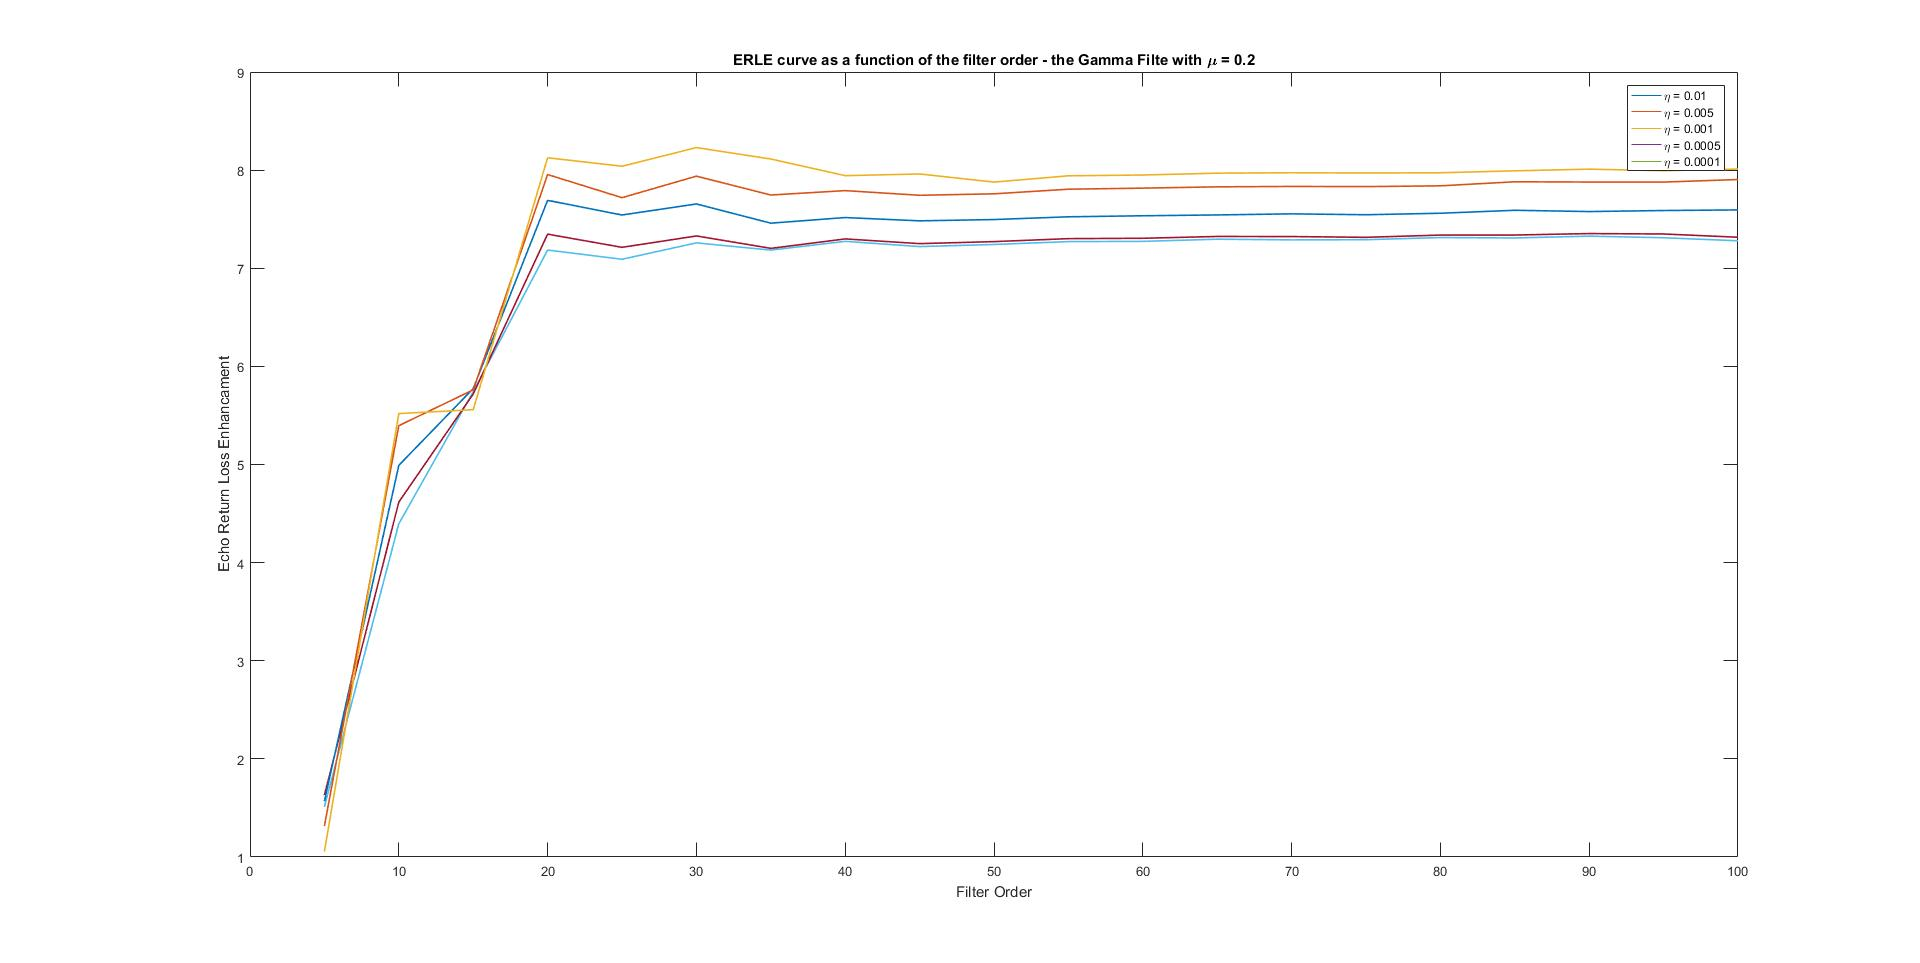
\includegraphics[width=3in]{GammaERLEaLL.jpg}}
	\caption{The ERLE curve of the Gamma filter after adaptation as a function of the number of taps with different step sizes $\eta$. With $\eta = 0.01$, the ERLE gains its maximum 7.3272 when filter order is 90. With $\eta = 0.005$, the ERLE gains its maximum 7.3543 when filter order is 90. With $\eta = 0.001$, the ERLE gains its maximum 7.6920 when filter order is 20. With $\eta = 0.0005$, the ERLE gains its maximum 7.9549 when filter order is 20. With $\eta = 0.0001$, the ERLE gains its maximum 8.2298 when filter order is 30.}
	\label{ERLEGammaall}
	\end{figure}
	
	%\begin{table}[htbp]
	%\centering 
	%\begin{tabular}{lccc}  
	%\hline
	%Step size & Optimal filter order & Maximum ERLE\\ \hline 
	%0.01 & 90 & 7.3272\\  
	%0.005 & 90 & 7.3543\\ 
	%0.001 & 20 & 7.6920\\ 
	%0.0005 & 20 & 7.9549\\ 
	%50.0001 & 30 &8.22987\\ \hline
	%\end{tabular}
	%\caption{Comparison of LMS filter result with different step size.}
	%\end{table}
	
	Based on the results shown above, we can conclude that even we have different optimal filter order when using different step size $\eta$ with fixed feedback parameter $\mu$, the ERLE value tend to not change much from about filter order 20. And also by listening to the result, I found that with filter order 30 and larger, our ears will not be able to hear any difference. And that at filter order 30 to 40, the recovered speech appears to be much clearer compared to others.
	
	Hoping to find the best feedback parameter $\mu$ for the gamma filter, I changed the filter order from 20 to 50, and with every filter order fixed,  I changed $\mu$ from 0 to 1 in steps of 0.05. And the step size are chosen to be 0.005.  For every single filter order being tested on, they perform best when the feedback parameter $\mu = 0.15$ or $\mu = 0.2$. For example, the best feedback parameter $\mu$ for filter order 30 is 0.2. 
	\begin{figure}[h]
	\centerline{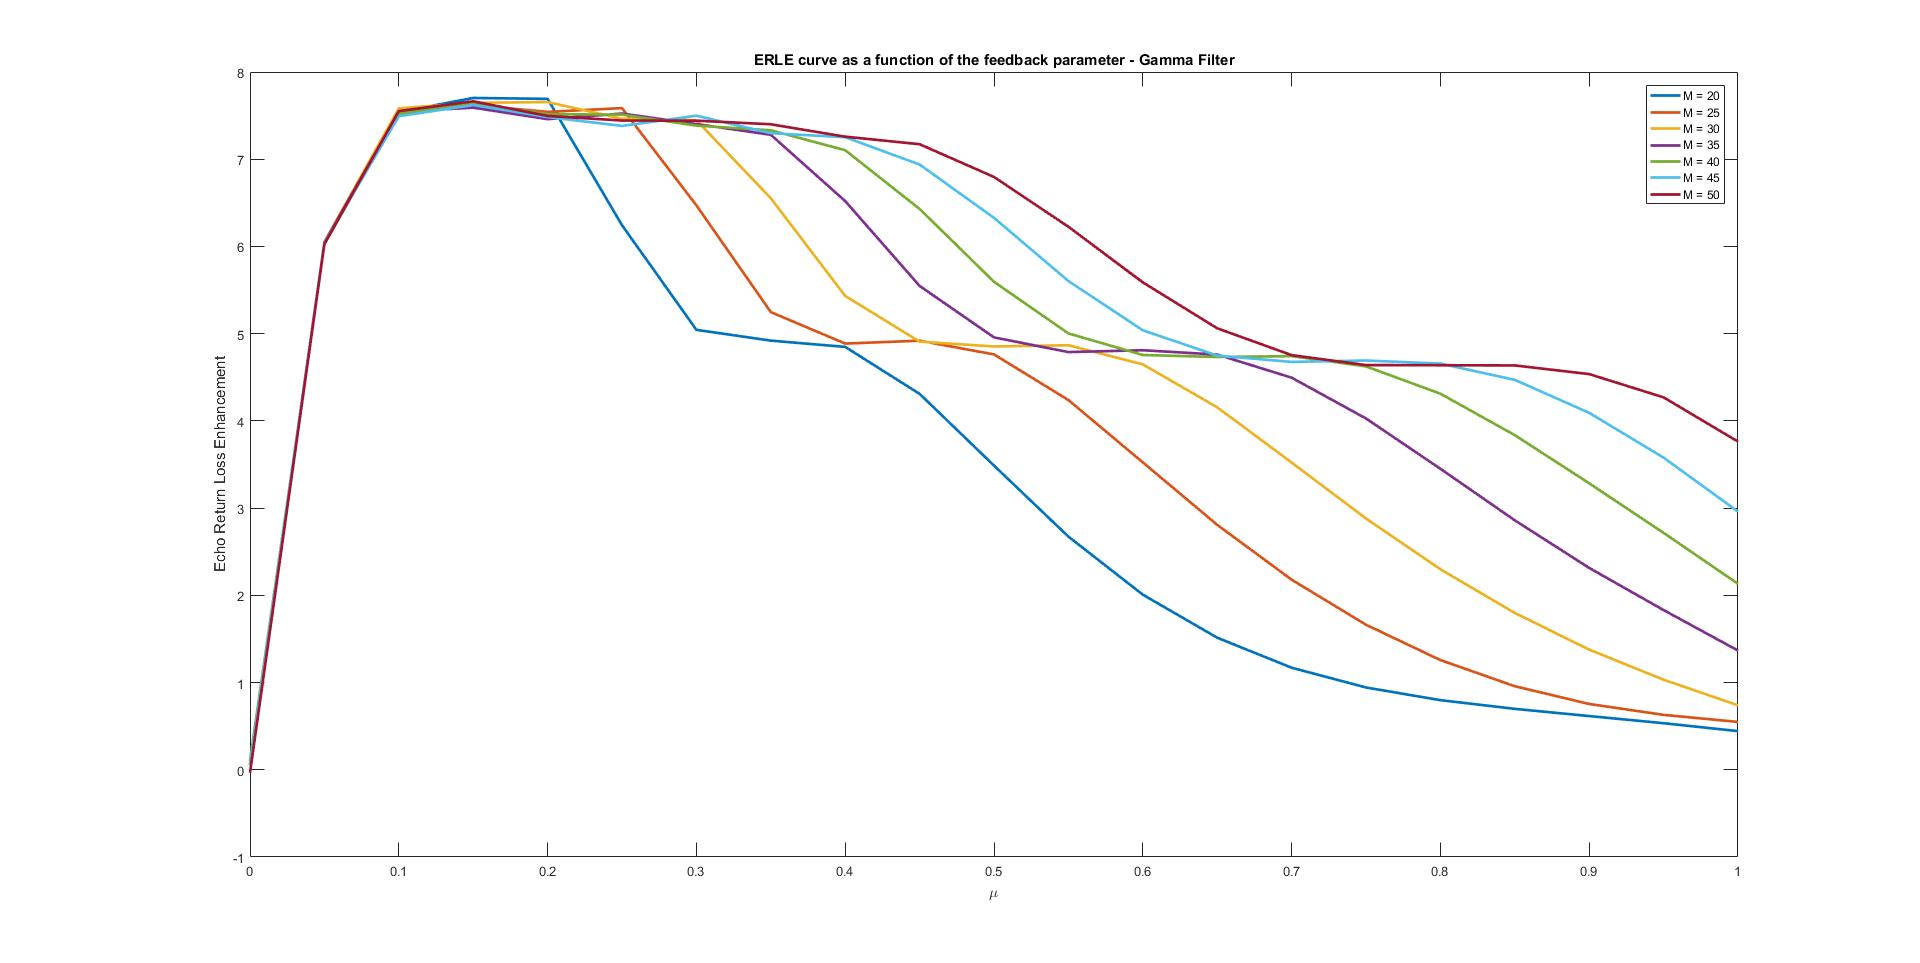
\includegraphics[width=3in]{ERLEcomparisonfor_bestmu_0001.jpg}}
	\caption{The comparison of ERLE curve of the Gamma filter after adaptation as a function of feedback parameter with $\eta = 0.005$.  The ERLE gains its maximum 7.7022 when filter order is 20, feedback parameter $\mu$ is 0.15}
	\label{ERLEComp}
	\end{figure}

	For a Gamma filter with fixed feedback parameter $\mu = 0.15$ and fixed filter order 30, the learning curve and weight track is examined. Figure \ref{LCGammaAll} shows the learning curves with different step sizes in one plot.
Figures \ref{gammaLCWT1} to \ref{gammaLCWT5} show the selected weight tracks with different learning step sizes. 


	\begin{figure}[htbp]
	\centerline{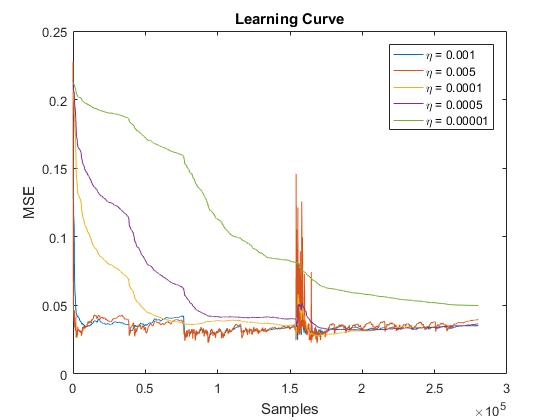
\includegraphics[width=2.5in]{Gamma_LC_all_mu15_M30.jpg}}
	\caption{The comparison of learning curves of the Gamma filter the number of taps 30 and  $\eta =10^{-5}$.}
	\label{LCGammaAll}
	\end{figure}	

	\begin{figure}[htbp]
	\centering
	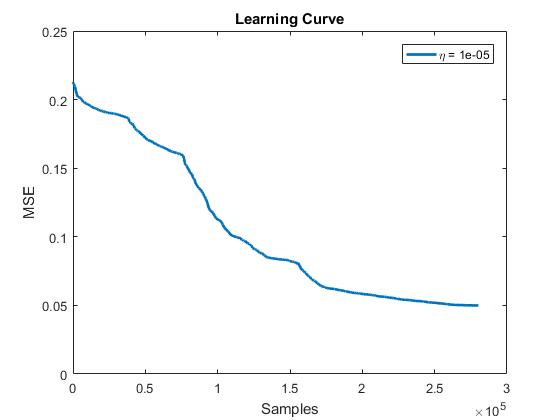
\includegraphics[width = 1.7in]{Gamma_LC_eta5_mu15_M30.jpg}
	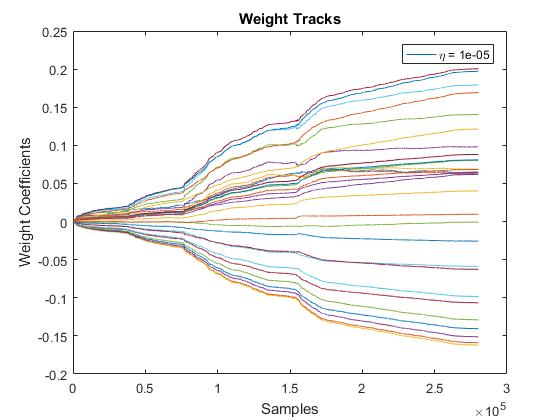
\includegraphics[width=1.7in]{Gamma_WT_eta1_mu15_M30.jpg}
	\caption{Left: The learning curve of the Gamma filter with number of taps 30 and  $\eta =10^{-5}$. Right: The weight track of the Gamma filter with number of taps 30 and  $\eta = 10^{-5}$.}
	\label{gammaLCWT1}
	\end{figure}

	\begin{figure}[htbp]
	\centering
	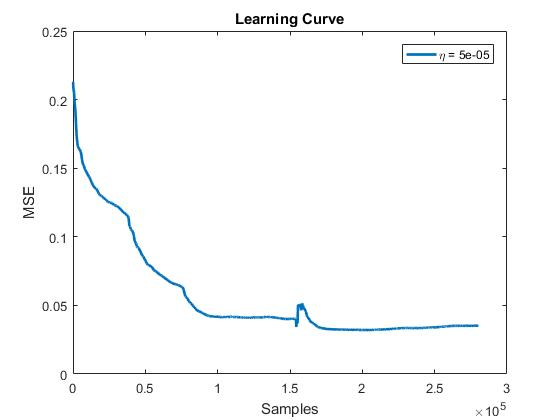
\includegraphics[width = 1.7in]{Gamma_LC_eta4_mu15_M30.jpg}
	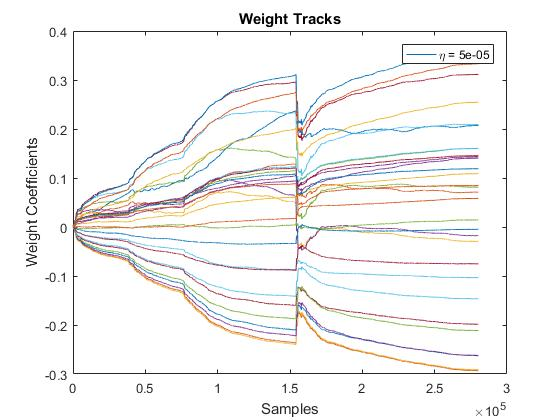
\includegraphics[width=1.7in]{Gamma_WT_eta2_mu15_M30.jpg}
	\caption{Left: The learning curve of the Gamma filter with number of taps 30 and  $\eta = 5\times 10^{-5}$. Right: The weight track of the Gamma filter with number of taps 30 and  $\eta =5\times 10^{-5}$.}
	\label{gammaLCWT2}
	\end{figure}


	\begin{figure}[htbp]
	\centering
	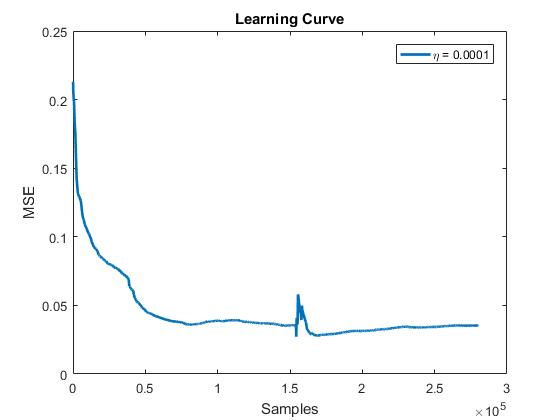
\includegraphics[width = 1.7in]{Gamma_LC_eta3_mu15_M30.jpg}
	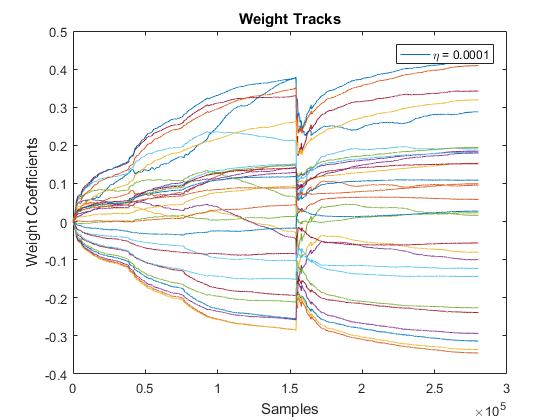
\includegraphics[width=1.7in]{Gamma_WT_eta3_mu15_M30.jpg}
	\caption{Left: The learning curve of the Gamma filter with number of taps 30 and  $\eta = 0.0001$. Right: The weight track of the Gamma filter with number of taps 30 and  $\eta = 0.0001$.}
	\label{gammaLCWT3}
	\end{figure}


	\begin{figure}[htbp]
	\centering
	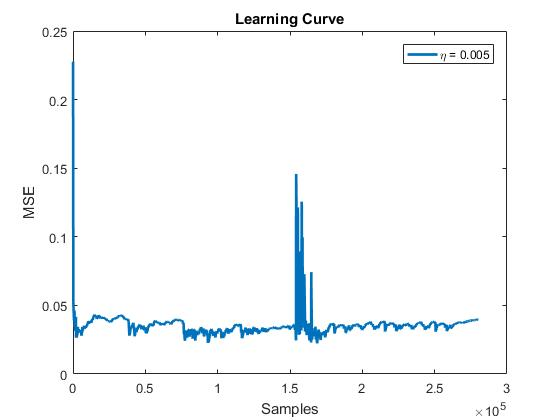
\includegraphics[width = 1.7in]{Gamma_LC_eta2_mu15_M30.jpg}
	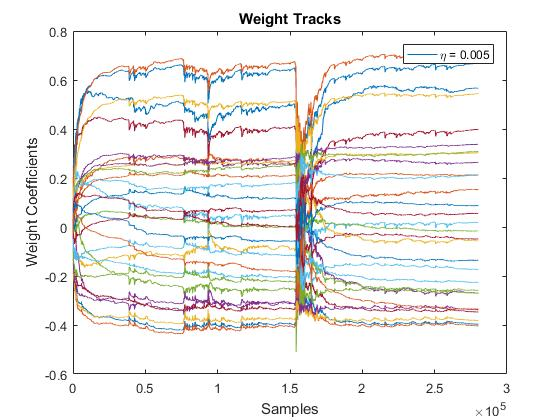
\includegraphics[width=1.7in]{Gamma_WT_eta4_mu15_M30.jpg}
	\caption{Left: The learning curve of the Gamma filter with number of taps 30 and  $\eta =0.005$. Right: The weight track of the Gamma filter with number of taps 30 and  $\eta = 0.005$.}
	\label{gammaLCWT4}
	\end{figure}


	\begin{figure}[htbp]
	\centering
	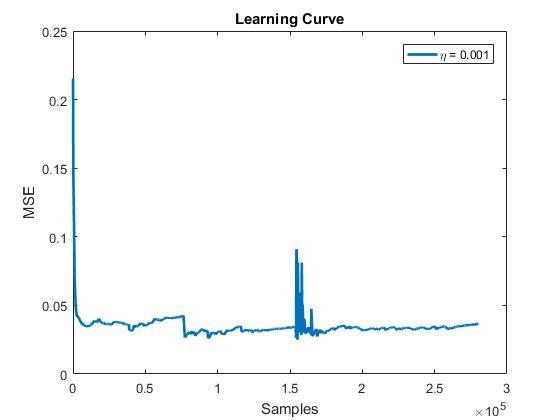
\includegraphics[width = 1.7in]{Gamma_LC_eta1_mu15_M30.jpg}
	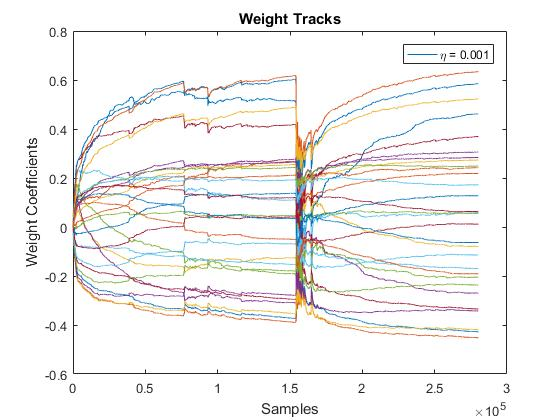
\includegraphics[width=1.7in]{GammaWT_eta5_mu15_M30.jpg}
	\caption{Left: The learning curve of the Gamma filter with number of taps 30 and  $\eta =0.001$. Right: The weight track of the Gamma filter with number of taps 30 and  $\eta = 0.001$.}
	\label{gammaLCWT5}
	\end{figure}


\section{Discussion}
	The plots of comparison of the recovered speech and the corrupted speech obtained with all three filters are shown in figures \ref{comWiener} to \ref{comGamma}.
	\begin{figure}[htbp]
	\centerline{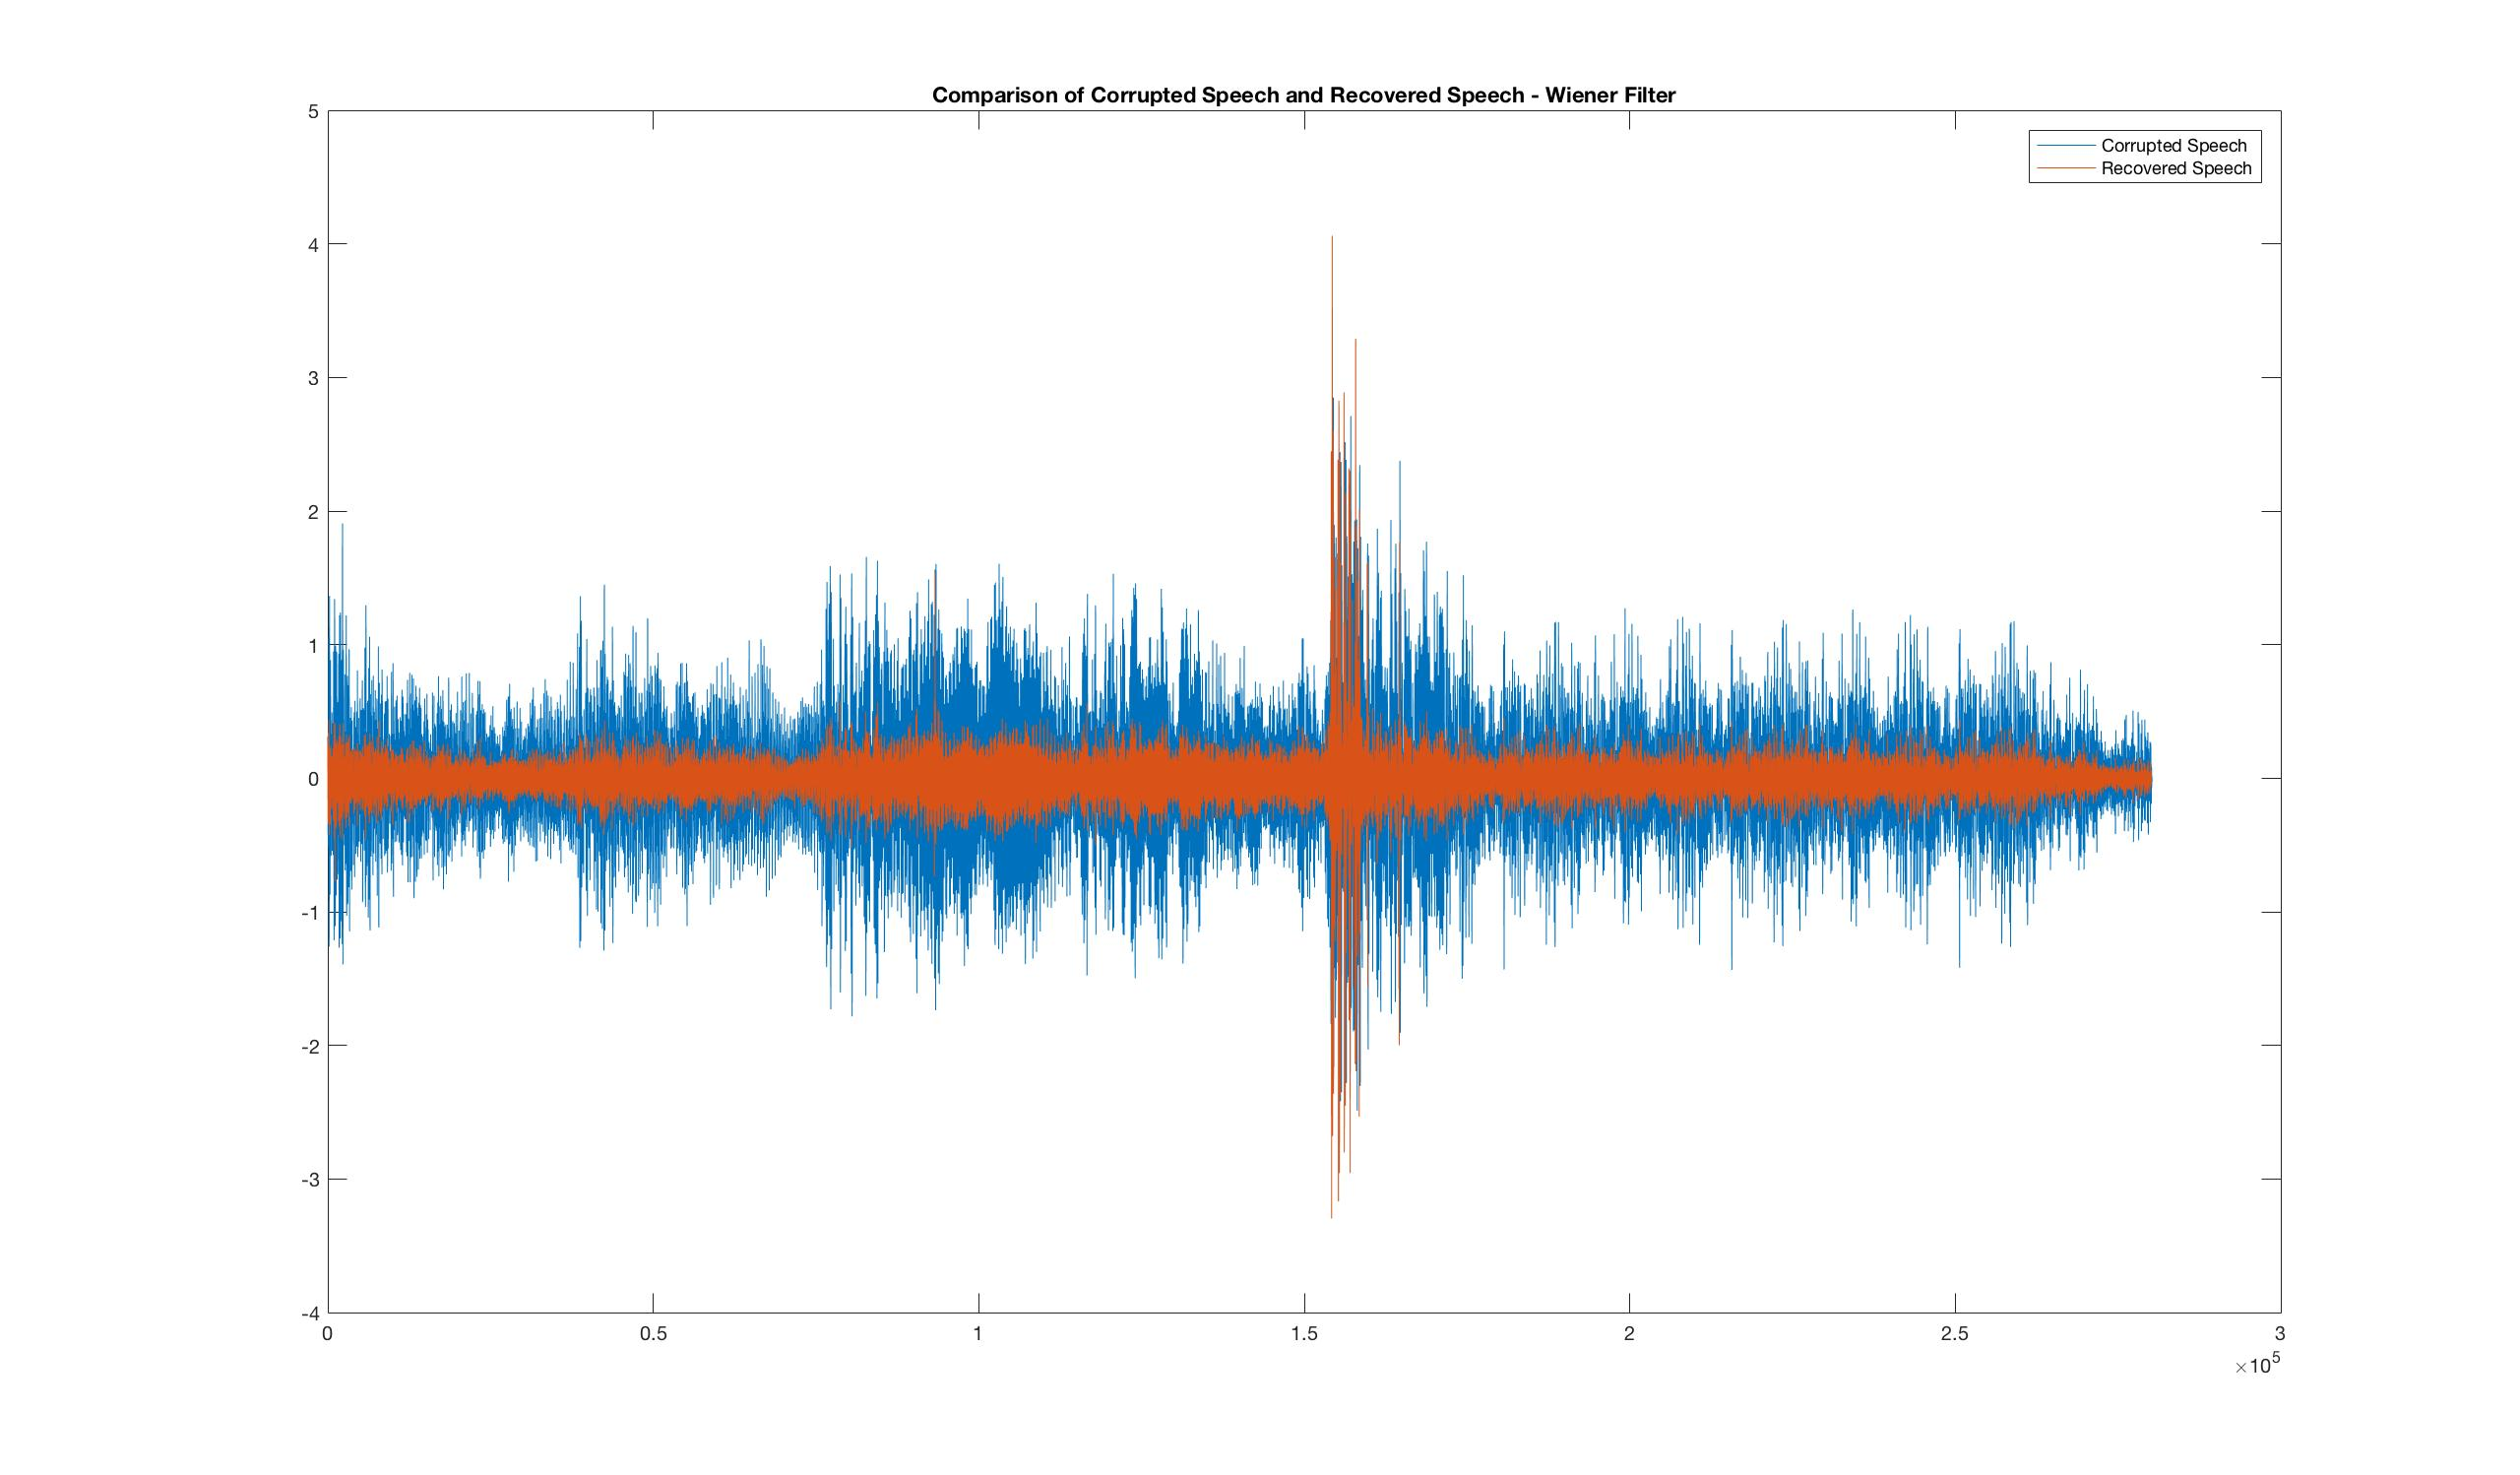
\includegraphics[width=3.5in]{WienerComparison.jpg}}
	\caption{The comparison of corrupted and recovered speech - the Wiener filter}
	\label{comWiener}
	\end{figure}	
	\begin{figure}[htbp]
	\centerline{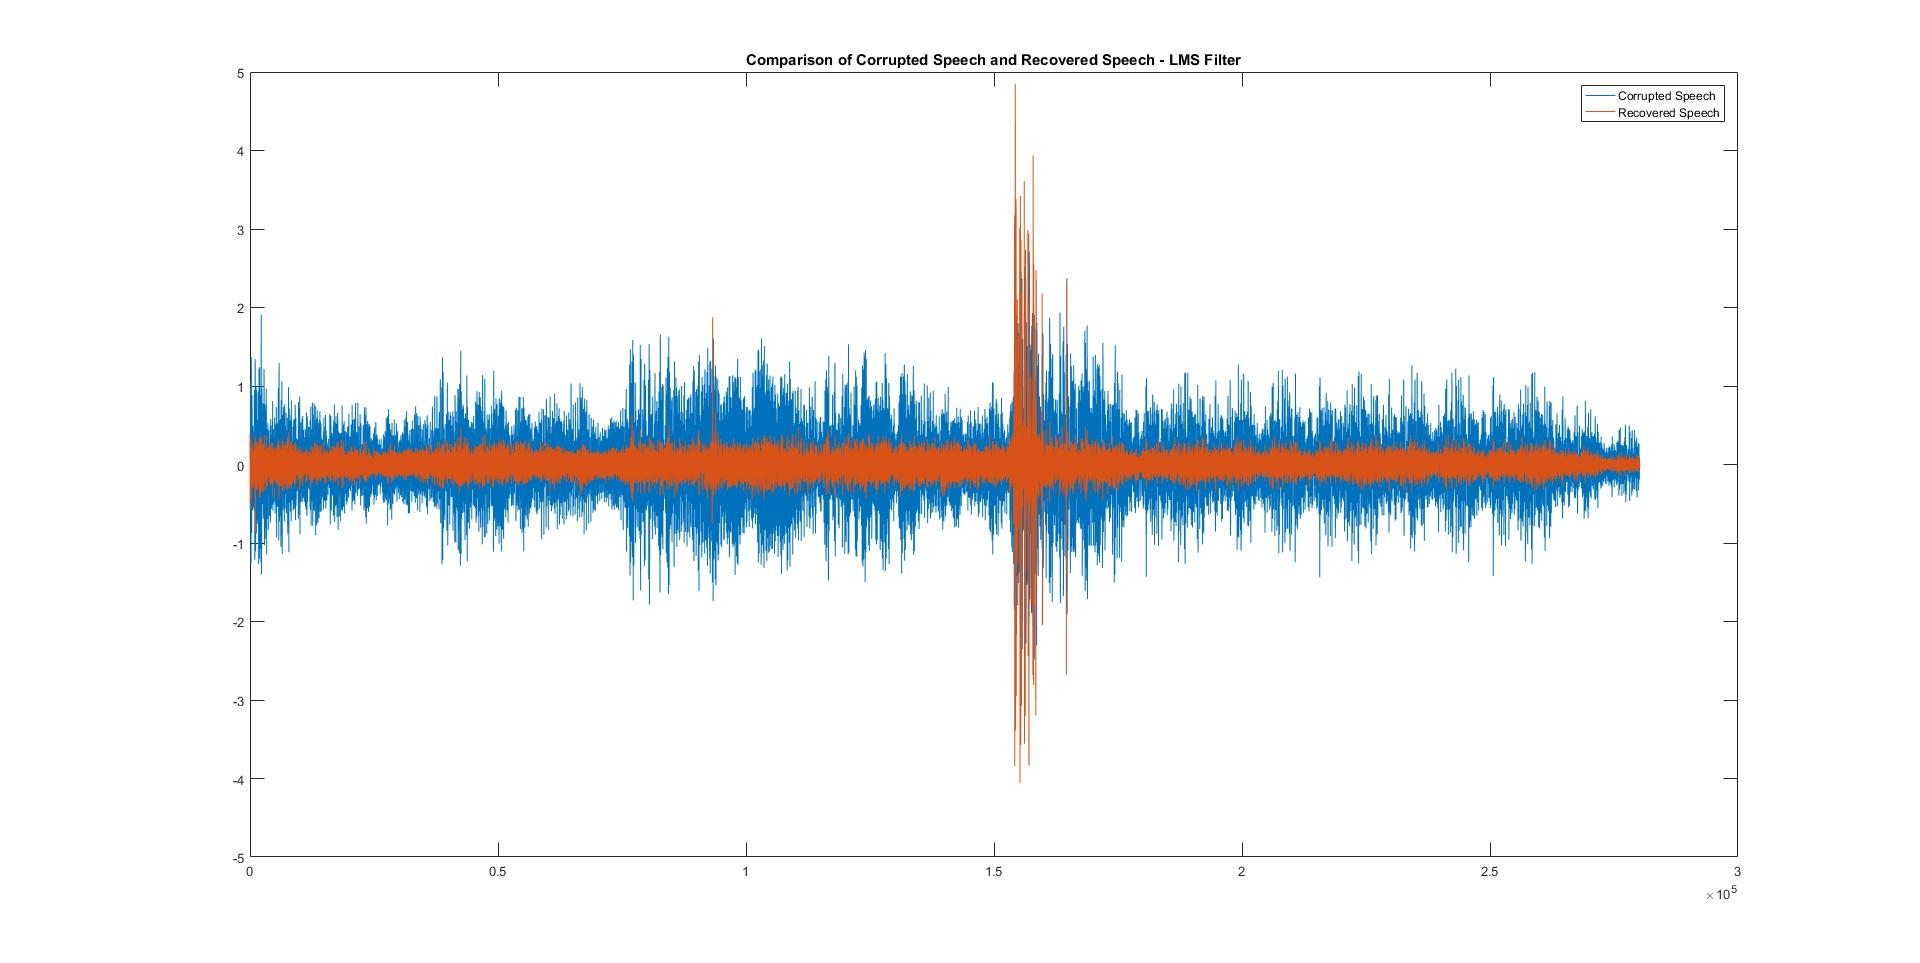
\includegraphics[width=3.5in]{LMScomparison.jpg}}
	\caption{The comparison of corrupted and recovered speech after 200 iteration over all samples - the LMS filter.}
	\label{comGamma}
	\end{figure}
	\begin{figure}[htbp]
	\centerline{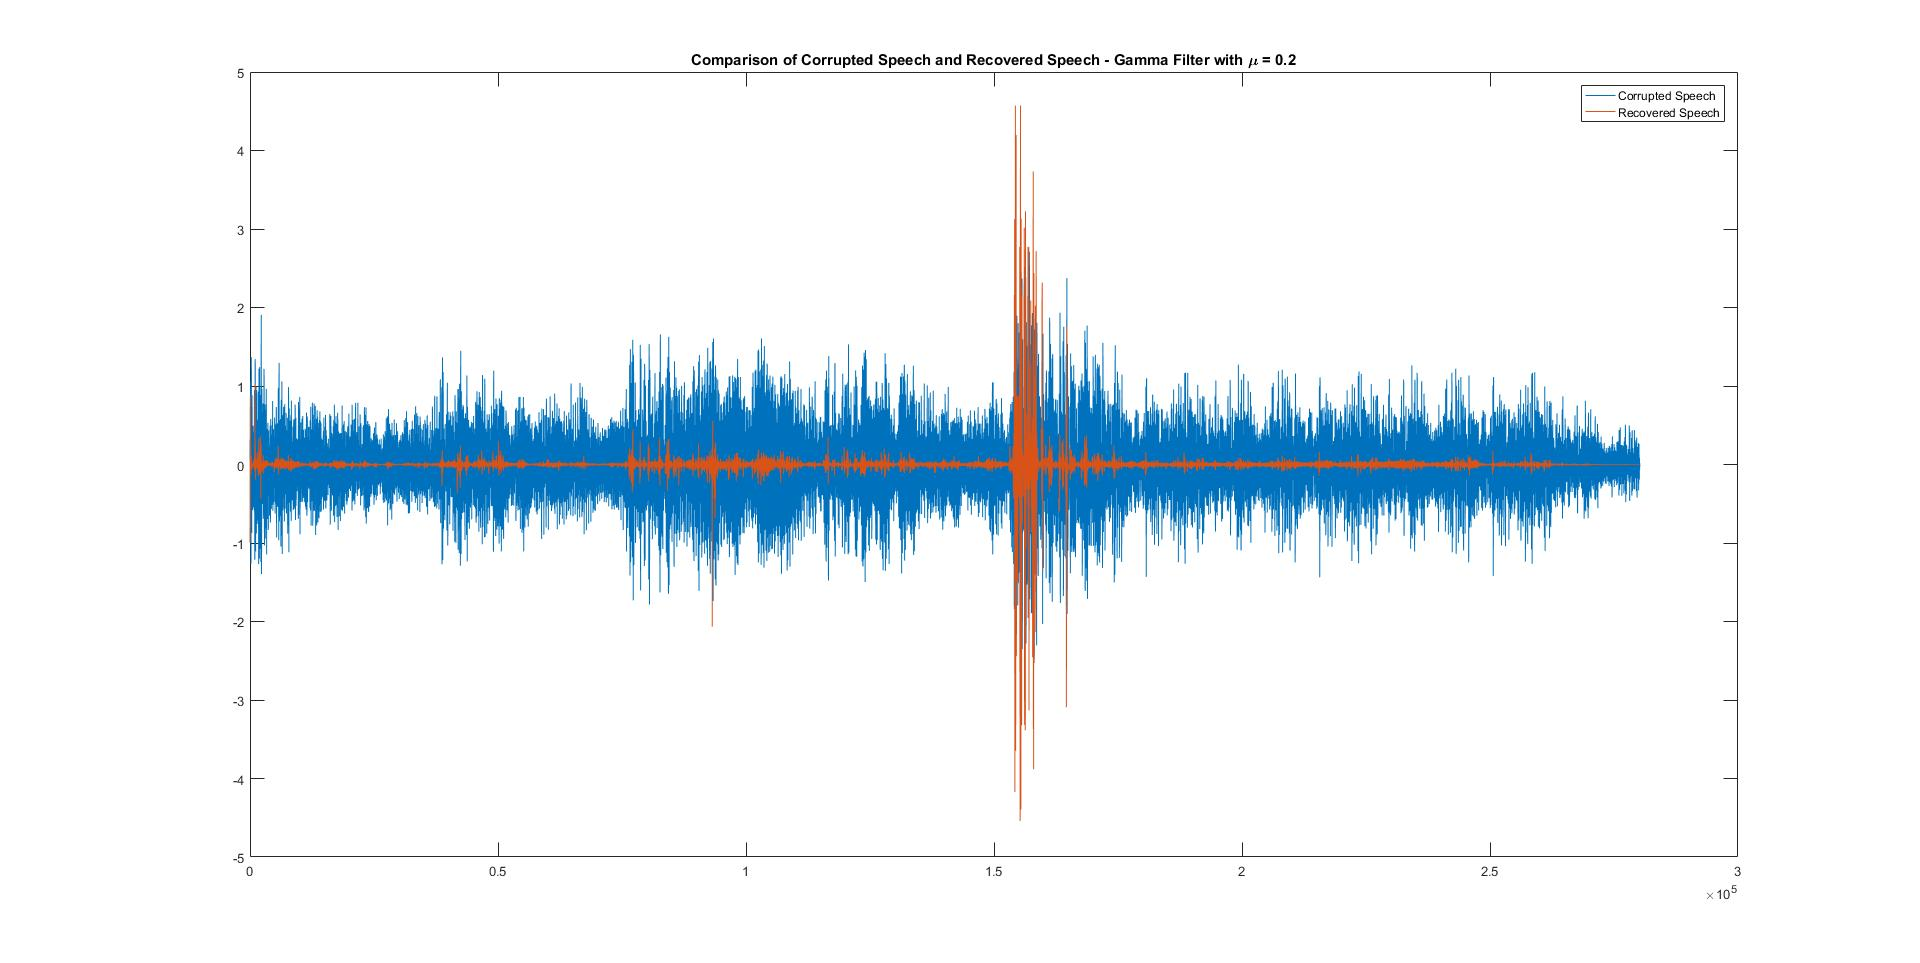
\includegraphics[width=3.5in]{Gamma_eta001_mu02.jpg}}
	\caption{The comparison of corrupted and recovered speech - the Gamma filter.}
	\label{comGamma}
	\end{figure}
	If we look at the result gained by the Wiener solution of the FIR filter,  we can see that the Wiener solution is not suitable for the non-stationary problem we are dealing with - as shown in figure \ref{fig2}, for 2 randomly chosen windows, the calculated weight coefficient differs a lot. Also, when listen to the ``recovered speech", it does not sounds like recovered at all - it sounds like almost the same as the corrupted one, although the Wiener filter obtains a comparatively high value of ERLE 8.3208. And since Wiener solution is an analytical solution, there is nothing to do to improve the result.

	Since the Wiener solution is not suitable for the non-stationary problem, one may consider the online learning method - the LMS solution of the FIR filter.  When we examine the results with the LMS filter, based on the ERLE measure, the best performance is with large filters (close to 100) and small step size (e.g. $10^{-5}$). While if listen to the recovered speech, it still cannot get a clear speech. Actually, the result of LMS filter would not have big changed even after 200 iterations of all the samples.
	
	If trying to solve this problem with an IIR filter, i.e. the Gamma filter in this case, the results show that the filter with filter order at around 30 and the feedback parameter $\mu$ at around 0.2 gives the best performance. As mentioned before, the value of ERLE barely change when filter order is greater than 30, especially when comparing by listening.

	For the two online learning methods, when examining the learning curves, we get the learning behaviours for both of them. The learning curves for LMS filter and the Gamma filter are shown in figures \ref{LMSlcALL} and \ref{LCGammaAll} respectively. If we look at figure \ref{LMSlcALL}, we would see that when the step size is too large, e.g. $\eta = 0.001$, the error term keeps boucing up and down, which means keeps searching for the solution while not converge and may never converge. And at about the half of the learning precedure, there is a point where the curve changes suddenly if the step size is too large. This may be explained by the inflection point in the original signal at about the same place.When it comes to learn the weights to best estimates the signal at that place, using a large step size would cause the error term to change significantly suddently at that point, and thus the weight coefficients also change significantly suddently at the same place. And this sudden change on weight coefficients would again cause a larger mean squared error. That also explains we see sudden changes in the weight tracks shown in \ref{LMSeta1} to \ref{LMSeta6} as well as \ref{gammaLCWT1} to \ref{gammaLCWT5} . Conversely, if a small step size is chosen, which means the learning procedure is rather slow - the weight coefficients change only a little bit at every step, and thus causes fail to converge in specific iterations. In other words, it takes a longer time to converge. This phenomenon can also be observed in the weight tracks, when using a small step size, the weight coefficients change a little bit at a time, but the learning procedure is a rather smooth, causing a long time to converge. 

	When compare two online learning methods, the LMS filter is unable to get a good result even if the whole procedure is repeated 200 times, while it is rather easier for the Gamma filter to get a rather clear recovered speech within a short time. This may result form the way the how the two filters work. Figure \ref{gamma100} shows the result of the Gamma filter with the same filter order with the LMS filter, i.e. $M = 100$. Comparing the figures \ref{comGamma} and \ref{gamma100}, we can see that obviously the Gamma filter has a much better result; and if measured by listening to the result, the Gamma filter removes almost all the music, gives us a speech with some noise, while the LMS filter fails to even remove all the music. I can only here a little bit speech at the very end of the voice.
	\begin{figure}[htbp]
	\centerline{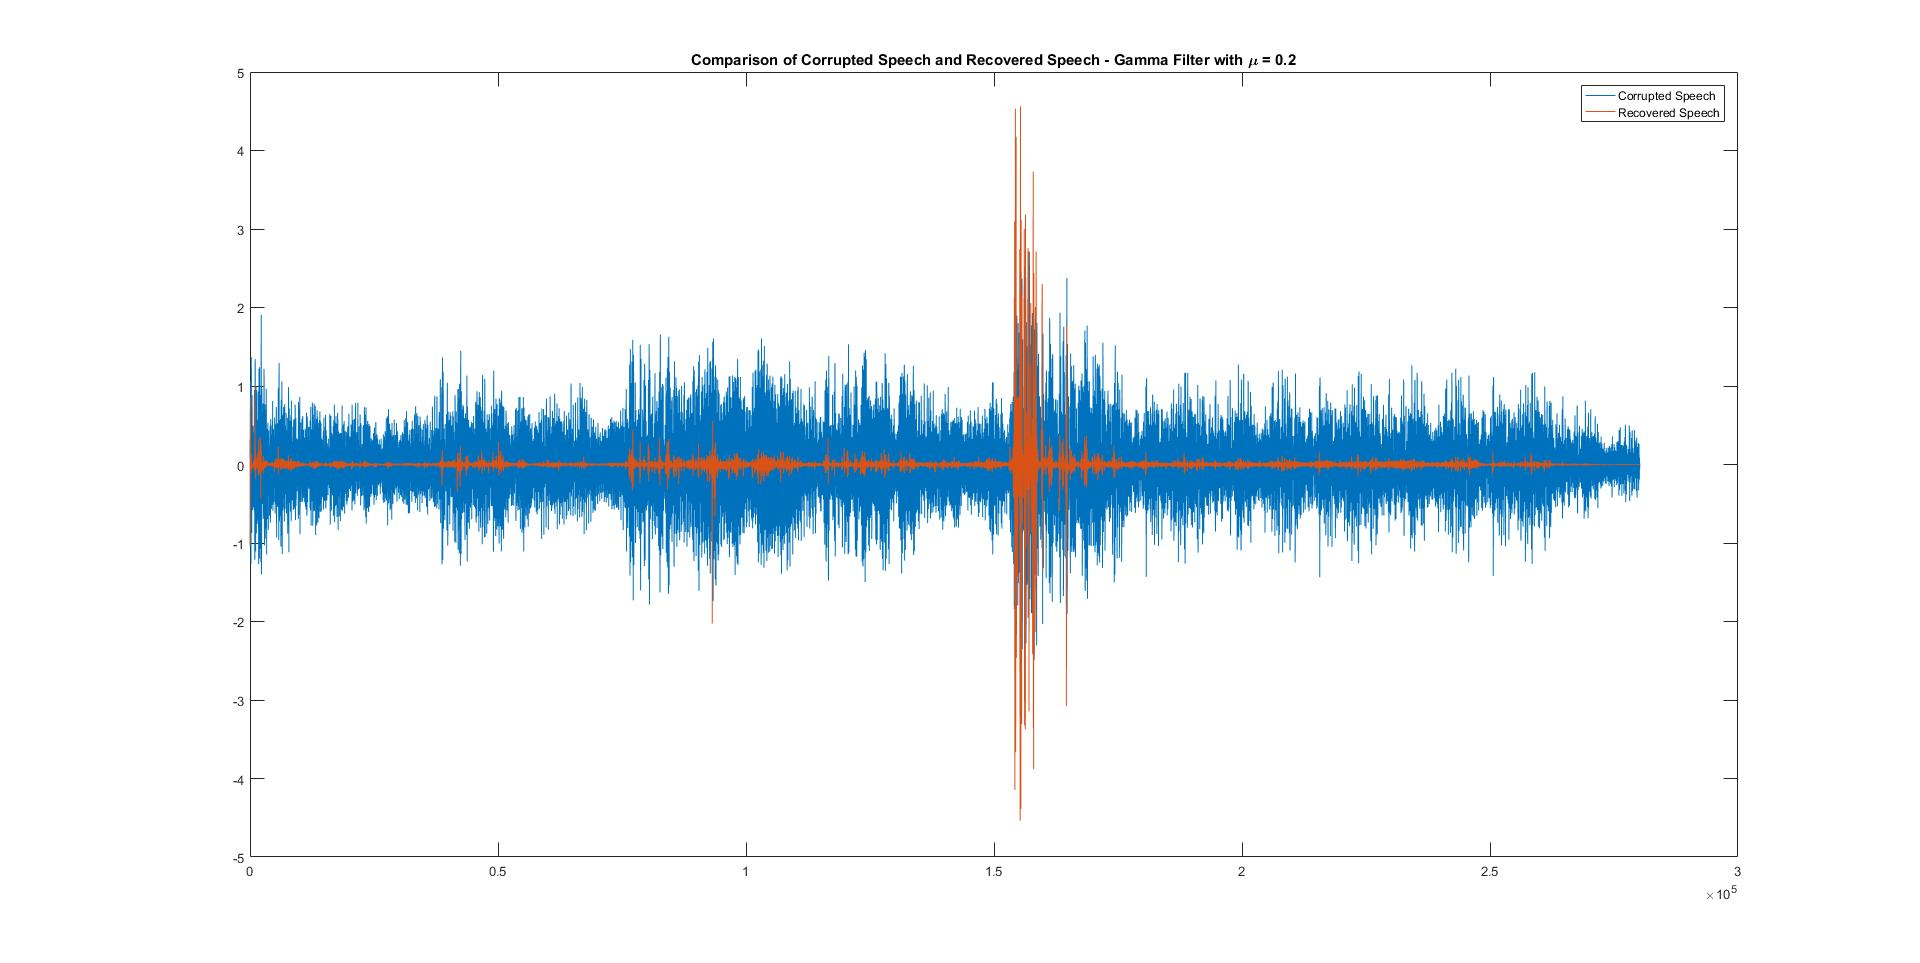
\includegraphics[width=3.5in]{Gamma_eta0005_mu02_M100.jpg}}
	\caption{The comparison of corrupted and recovered speech - the Gamma filter with the same filter order 100.}
	\label{gamma100}
	\end{figure}

\section{Conclusions}  For this specific problem we are dealing with, because of its non-stationarity, it is not suitable to use the Wiener solution of FIR filter; with the ability to update weight coefficient locally, least mean square filter and the Gamma filter would be suitable for this problem. 

	When looking at the learning curves and the weights for both LMS filter and the Gamma filter, we can conclude that both of them need to make compromise when choosing step sizes: neither too small to converge to slow, nor too large to unable to converge. And for both the learning curves and the weight tracks we may find a ``strange" point where the curve changes suddenly.  Having the same inflection point in the original signal explains this. As stated above in the discussion, both the LMS filter and the Gamma filter should work, but when comparing them, the Gamma filter performs much better in this problem - using the same filter and the learning rate, the Gamma filter is able to recover the speech with only one iteration while the LMS can only remove a little of the music after several iterations. Which indicates this signal is of memory related - the filter with better memory characteristic performs better.
	
	While conceptually both LMS solution with FIR filters and the Gamma filters should work, the results of my experiments show that the Gamma filters work much better. Since the echo formation would be a complicated procedure, thus filters with feedback like the Gamma filter may perform better because of the characteristic of deep memory. For the Gamma filters, the best filter orders are around 30, and the best feedback parameters are around 0.2.

	The best recovered speech gained by the Gamma filter eliminates almost all the music, makes us able to hear the words, but with some remaining noise. 

	The future works can be related to design non-linear filters which adapt online learning procedure, which may better mimic the way the echo forms.
	
	%Sometimes a large ERLE is got, but the sound is still not clear than some with smaller ERLE, examine the equation:$$ERLE = 10log_{10}\displaystyle\frac{\frac{1}{N}\sum_{i=1}^{N}d_i^2}{\frac{1}{N}\sum_{i=1}^{N}e_i^2} = 10log_{10}\displaystyle\frac{\sum_{i=1}^{N}d_i^2}{\sum_{i=1}^{N}e_i^2}$$
	%looking only at $\frac{\sum_{i=1}^{N}d_i^2}{\sum_{i=1}^{N}e_i^2}$, in our case, the desired part is a combination of desired speech and the echo, 

\begin{thebibliography}{00}
\bibitem{b1} https://en.wikipedia.org/wiki/Finite\_impulse\_response
\bibitem{b2} Elements of Machine Intelligence lecture notes.
\bibitem{b3} Principe, Jose C., Euliano Neil R. and Lefebvre W. Curt. ``Neural and Adaptive Systems: Fundamentals through Simulations." (1991): 386-393.
\bibitem{b4}https://en.wikipedia.org/wiki/Infinite\_impulse\_response
\bibitem{b5}Principe, Jose C., Bert De Vries, and Pedro Guedes De Oliveira. ``The gamma-filter-a new class of adaptice IIR filters with restricted feedback.\emph{" IEEE transactions on signal processing} 41.2 (1993): 649-656.
\end{thebibliography}

\emph{I confirm that this assignment is my own work, is not copied from any other's work (published or unblished), and has not been previously submitted for assessment either at University of Florida or elsewhere.}
	\begin{figure}[htbp]
	\centerline{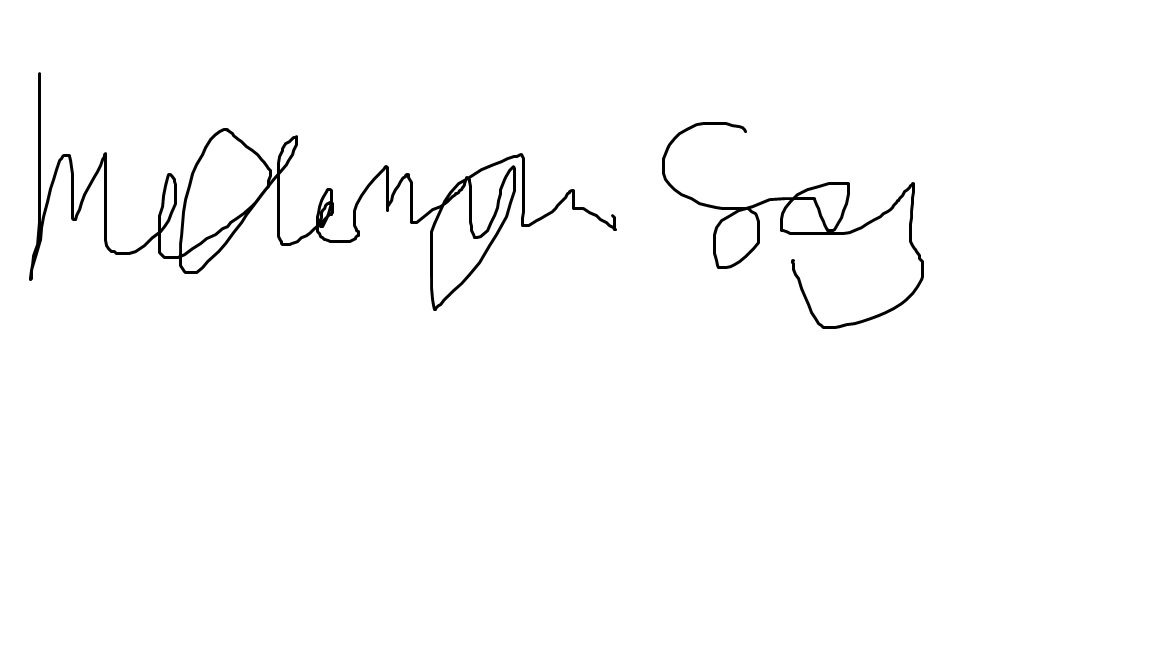
\includegraphics[width=3.5in]{sig.jpg}}

	\label{gamma100}
	\end{figure}

\end{document}
